
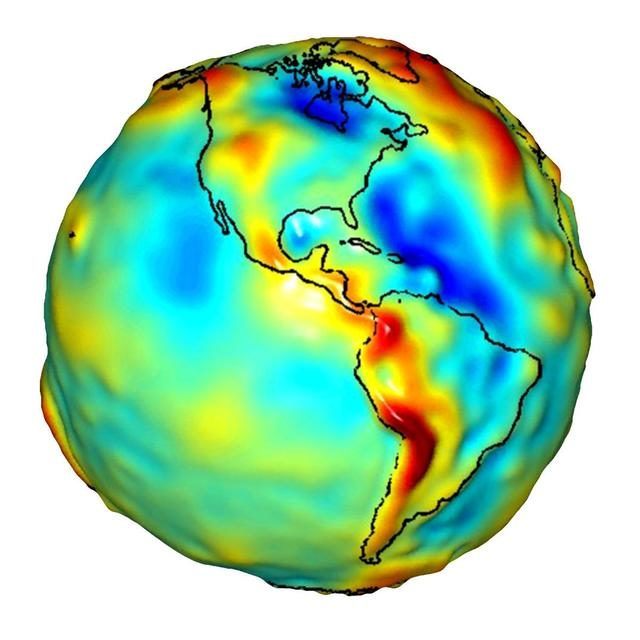
\includegraphics[height=1.5cm]{images/pictograms/gravity}

%\lstinputlisting[language=bash,basicstyle=\small]{python_codes/fieldstone_113/keywords.ascii}

\begin{center}
\inpython~Code at \url{https://github.com/cedrict/fieldstone/tree/master/python_codes/fieldstone_113}
\end{center}

\par\noindent\rule{\textwidth}{0.4pt}

%%%%%%%%%%%%%%%%%%%%%%%%%%%%%%%%%%%%%%%%%%%%%%%%%%%%%%%%%%%%%%%%%%%%%%%%%%%%%%%%%%%%%%%%%%%%%%%%%%%%

Last revision: Sept. 26th, 2024.

\par\noindent\rule{\textwidth}{0.4pt}
%%%%%%%%%%%%%%%%%%%%%%%%%%%%%%%%%%%%%%%%%%%%%%%%%%%%%%%%%%%%%%%%%%%%%%%%%%%%%%%%%%%%%%%

Note that there are two python files in the folder: {\python stone\_tetrahedron.py}
and {\python stone\_hexahedron.py}.

This \stone based on the article by Werner \& Scheeres (1997) \cite{wesc97} in which 
the gravity fields generated by a polyhedron {\it of constant density}.

Before we dive in the calculations it is worth highlighting a few excerpts from the paper. 
First, the authors present three methods to compute the gravity field of an irregular-shaped
body:
\begin{enumerate}
\item harmonic expansion. They write:
\begin{displayquote}
{\color{darkgray}
Harmonic expansions have several drawbacks. 
The first is that the harmonic expansion is always an approximation to a gravity field due to the finite
truncation of the series expansion. The truncation error grows when evaluating
the gravity field close to the model's radius of convergence. Additional terms are
necessary in the expansion to maintain a given accuracy.\\
The second major drawback is that the same form of the exterior harmonic
expansion is no longer guaranteed to converge inside the circumscribing sphere,
and indeed often diverges.\\
Another drawback is that the harmonic expansion yields no information about
whether a field point is outside or inside the body.}
\end{displayquote}

\item mass concentrations ('mascons').

\begin{displayquote}
{\color{darkgray}
A second, commonly used approach for evaluating asteroid gravitation is to fill the
body with point masses ('mascons' - mass concentrations) on an evenly spaced
grid (Geissler et al., 1995).
[...] for a given computational effort, the mascon approach is less accurate than 
a harmonic approach (in its region of convergence).}
\end{displayquote}


\item polyhedron. This is the method presented in the paper. 
\begin{displayquote}
{\color{darkgray}
we investigate a third approach, which is to model the asteroid as a
constant-density polyhedron. The polyhedron can have concavities in its surface
(e.g. craters), overhangs, interior voids (caves), and even holes all the way through
(torus). There is no special penalty for including small details, i.e. the entire body
does not have to be modeled at a uniformly high resolution.
[...] The polyhedral approach remedies several drawbacks outlined above.
The gravity field is exact for the given shape and density.
polyhedron gravitation is a valid and exact solution up to the surface of
the body. There is no region of divergence.
[...] Another way our work differs is that our ultimate formulas are expressed intrinsi-
cally using vectors and distances. Other papers are cluttered with special coordinate
systems and angles.
}
\end{displayquote}

\end{enumerate}


The authors explain what a polyhedron is in this context:
\begin{displayquote}
{\color{darkgray}
By polyhedron we mean a three-dimensional solid body whose surface consists of planar faces 
meeting along straight edges or at isolated points called vertices. Exactly two faces meet 
at each edge. Three or more edges and a like number of faces meet at each vertex. Note: 
the vertex coordinates of a polyhedron alone are insufficient to describe it. The connective 
topology must also be described -- edges connect which vertex pairs and bound which face pairs.}
\end{displayquote}

The volume integrals are transformed via the Gauss divergence theorem, into surface integrals, e.g.:
\[
U = \frac12 {\cal G} \rho_0 \iint_S \vec{n} \cdot \frac{\vec{r}}{r} \; dS
\]
Ultimately this integral will involve face integrals and edges integrals.
The paper is somewhat complex but well written. There is however no point re-typing all 
the derivations and I present in the next section the finalised equations of their Section~2.6.


%--------------------------------------------------------
\section*{Tetrahedron: the theory}

In what follows $e=1,2,...6$ stands for an edge while $f=1,2,3,4$ stands
for a face. 
Each polyhedron face has an outward-pointing face normal vector $\vec{n}_f$
and a face dyad ${\bm F}_f =\vec{n}_f\vec{n}_f $.
Each edge of each face has an outward-pointing edge normal
vector $\vec{n}_{e,f}$ perpendicular to both $\vec{n}_f$ and the edge.
For the edge connecting vertices 1 and 2 shared by faces A and B,
the edge dyad is ${\bm E}_{12}=\vec{n}_A \vec{n}_{12,A}+\vec{n}_B \vec{n}_{21,B}$.

Let $\vec{r}_i$ represent the vector from the variable 
field-point M at location $\vec{r}_M$ to polyhedron vertex $P_i$, 
and let $r_i = ||\vec{r}_i||$ be its length.


For the polyhedron edge connecting
vertices $i$ and $j$ of length $l_{ij}$, the dimensionless per-edge factor $L_e$ is
\[
L_e=L_{ij} = \int_e \frac{1}{r}ds = \int_{P_i}^{P_j} \frac{1}{r} ds 
= \ln \frac{r_i+r_j+l_{ij}}{r_i+r_j-l_{ij}}
\]
For a triangular face $f$ bounded by vertices $i,j,k$ the dimensionless
per-face factor $\omega_f$ is 
\[
\omega_f = 
\iint_{triangle} \frac{\Delta z}{r^3} dS 
= 2 \arctan \frac{\vec{r_i} \cdot (\vec{r}_j \times \vec{r}_k)}{r_ir_jr_k 
+r_i(\vec{r}_j\cdot\vec{r}_k) 
+r_j(\vec{r}_k\cdot\vec{r}_i) 
+r_k(\vec{r}_i\cdot\vec{r}_j) 
}
\]
The gravity vector $\vec{g}$ generated by the mass inside the tetrahedron 
at point $M$ is given by
\[
-\vec{g} = \vec\nabla U = 
- \underbrace{{\cal G} \rho_0 \sum_e L_e {\bm E}_e\cdot\vec{r}_e}_{\vec{g}_e}
+
\underbrace{{\cal G} \rho_0 \sum_f \omega_f {\bm F}_f\cdot \vec{r}_f}_{\vec{g}_f}
= -\vec{g}_e + \vec{g}_f
\]
with
\begin{eqnarray}
\vec{g}_e 
&=& {\cal G} \rho_0 \sum_e L_e {\bm E}_e \cdot \vec{r}_e \nn\\
&=& {\cal G} \rho_0 \left(
L_{12} {\bm E}_{12}\cdot\vec{r}_{12} +
L_{13} {\bm E}_{23}\cdot\vec{r}_{13} +
L_{14} {\bm E}_{34}\cdot\vec{r}_{14} \right. \nn\\
&& \left. + 
L_{23} {\bm E}_{23}\cdot\vec{r}_{23} + 
L_{24} {\bm E}_{24}\cdot\vec{r}_{24} +
L_{34} {\bm E}_{34}\cdot\vec{r}_{34} 
\right) \label{eq:tetra:ge}\\ \nn\\
\vec{g}_f
&=& {\cal G} \rho_0 \sum_f \omega_f {\bm F}_f\cdot \vec{r}_f \nn\\
&=& {\cal G} \rho_0 \left(
\omega_A {\bm F}_A\cdot \vec{r}_A +
\omega_B {\bm F}_B\cdot \vec{r}_B +
\omega_C {\bm F}_C\cdot \vec{r}_C +
\omega_D {\bm F}_D\cdot \vec{r}_D  
\right) \label{eq:tetra:gf}
\end{eqnarray}
and the gravity potential and tensor are then given by
\begin{eqnarray}
U &=& \frac12 {\cal G} \rho_0  \sum_e  L_e \; \vec{r}_e\cdot{\bm E}_e \cdot \vec{r}_e 
-\frac12 {\cal G} \rho_0 \sum_f \omega_f \; \vec{r}_f \cdot{\bm F}_f \cdot \vec{r}_f  \\
{\bm T} &=&
\vec\nabla\vec\nabla U = -\vec\nabla \vec{g} =
{\cal G} \rho_0 \sum_e 
L_e \cdot{\bm E}_e 
- {\cal G} \rho_0 \sum_f \omega_f \; {\bm F}_f 
\end{eqnarray}



Let us consider a generic tetrahedron:
\begin{center}
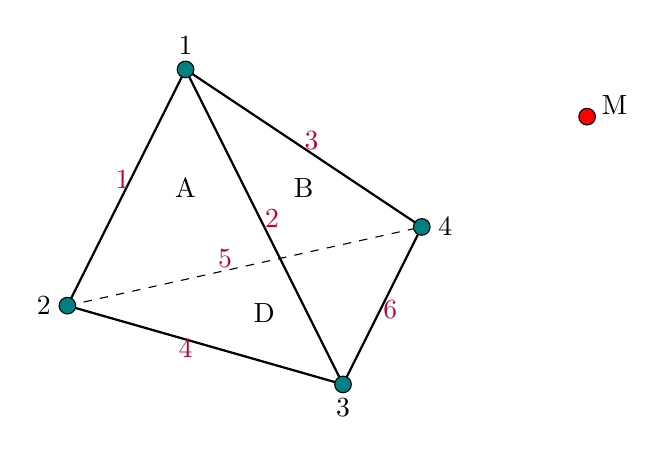
\begin{tikzpicture}
%\draw[step=0.5cm,gray,very thin] (0,0) grid (7,6); 
\draw[thick] (2.5,5) -- (1,2) -- (4.5,1) -- (5.5,3) -- cycle;
\draw[thick] (2.5,5)  -- (4.5,1) ;
\draw[dashed] (1,2) --  (5.5,3);
\node[] at (2.5,5.3) {$1$};
\node[] at (0.7,2) {$2$};
\node[] at (4.5,0.7) {$3$};
\node[] at (5.8,3) {$4$};
\draw[black,fill=teal] (2.5,5) circle (3pt);
\draw[black,fill=teal] (1,2) circle (3pt);
\draw[black,fill=teal] (4.5,1) circle (3pt);
\draw[black,fill=teal] (5.5,3) circle (3pt);
\node[] at (2.5,3.5) {A};
\node[] at (4,3.5) {B};
\node[] at (3.5,1.9) {D};
\draw[black,fill=red] (7.6,4.4) circle (3pt);
\node[] at (7.95,4.55) {M};
\node[] at (1.7,3.6) {\color{purple}1};
\node[] at (3.6,3.1) {\color{purple}2};
\node[] at (4.1,4.1) {\color{purple}3};
\node[] at (2.5,1.45) {\color{purple}4};
\node[] at (3,2.6) {\color{purple}5};
\node[] at (5.1,1.95) {\color{purple}6};
\end{tikzpicture}\\
{\captionfont Face C is hidden in the back.}
\end{center}


When looking at a face from the outside towards the tetrahedron the numbering 
of vertices is counter-clockwise.
\begin{center}
\begin{tabular}{ccccc}
\hline
face & vertices $i,j,k$ & edge \#1 & edge \#2 & edge \#3 \\
\hline\hline
A& 1,2,3  & 12({\color{purple}1}) & 23({\color{purple}4}) & 31({\color{purple}2}) \\
B& 1,3,4  & 13({\color{purple}2}) & 34({\color{purple}6}) & 41({\color{purple}3}) \\
C& 1,4,2  & 14({\color{purple}3}) & 42({\color{purple}5}) & 21({\color{purple}1}) \\
D& 2,4,3  & 24({\color{purple}5}) & 43({\color{purple}6}) & 32({\color{purple}4}) \\
\hline
edge & vertices & belongs to \\
{\color{purple}1} & 12 & A,C\\
{\color{purple}2} & 13 & A,B\\
{\color{purple}3} & 14 & B,C\\
{\color{purple}4} & 23 & A,D\\
{\color{purple}5} & 24 & C,D\\
{\color{purple}6} & 34 & B,D\\
\hline
\end{tabular}
\end{center}


\begin{center}
\begin{tikzpicture}
%\draw[step=0.5cm,gray,very thin] (0,0) grid (12,8.5); 
\draw[thick] (0.6,2.8) -- (3,5.6)--(6.7,6.9);
\draw[thick] (3,5.6)  -- (8.1,3.2) ;
\draw[thick] (5.9,0.4) -- (8.1,3.2) -- (11.1,4.2);
\node[] at (9,4.5) {face A};
\node[] at (4.5,2) {face B};
\draw[thick,->] (2.4,3.5)--(0.5,5); 
\node[] at (0.5,5.25) {$\vec{n}_B$};
\draw[] (2.2,3.65) -- (2.38,3.85) --(2.58,3.66);
\draw[thick,->] (5.5,5.7)--(5.2,8.1); 
\node[] at (5.6,8) {$\vec{n}_A$};
\draw[] (5.45,6) --(5.7,6.075) --(5.75,5.8);
\node[] at (2.7,5.7) {1};
\node[] at (8.2,2.85) {2};
\draw[black,fill=teal] (3,5.6) circle (3pt);
\draw[black,fill=teal] (8.1,3.2) circle (3pt);
\node[] at (8,5.8) {$\vec{n}_{21,B}$};
\draw[thick,->] (6.5,4)--(7.75,5.6); 
\node[] at (4,3) {$\vec{n}_{12,A}$};
\draw[thick,->] (6.5,4)--(4.1,3.2); 
\node[rotate=-25] at (5,5) {common edge};
\end{tikzpicture}\\
{\captionfont Figure made after Fig.~7 from \textcite{wesc97}.}
\end{center}



$\vec{n}_{1,A}=\vec{n}_{12,A}=(n_x,n_y)$ is such that it is perpendicular to $\vec{n}_A$ 
(it lies in the face $A$ plane), i.e. $\vec{n}_{1,A}\cdot \vec{n}_A=0$ and to edge $\#1$, i.e. 
$\vec{n}_{1,A}\cdot \vec{l}_{1}=0$. The cross product of $\vec{n}_A$ and $\vec{l}_{1}$ is 
by definition a vector perpendicular to both.
We also need to make sure it is pointing outwards. We then take the scalar product of a 
vector joining the center of the face and the middle of the 
edge under consideration. If it is negative then the normal is pointing towards the center of the 
face so it needs to be flipped.




%-------------------------------------------
\section*{Tetrahedron: Point mass approach}

Let us denote by $V$ the volume of the tetrahedron which 
can easily be computed:
\begin{equation}
V=\frac16 \left| (\vec{l}_{\color{purple}1} \times \vec{l}_{\color{purple}2}) \cdot \vec{l}_{\color{purple}3}\right|
\label{eq:tet:vol}
\end{equation}

\begin{center}
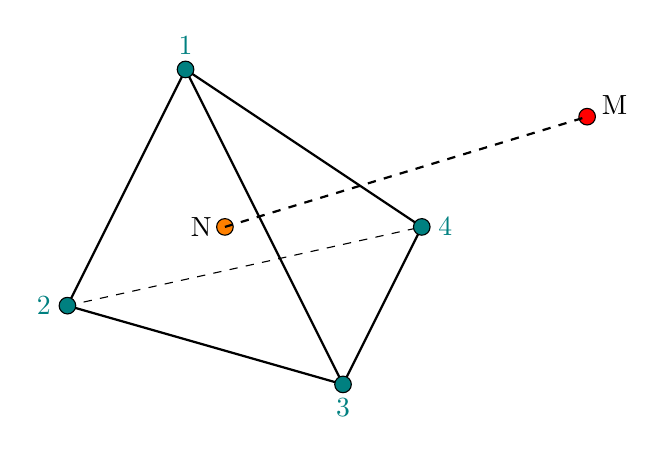
\begin{tikzpicture}
%\draw[step=0.5cm,gray,very thin] (0,0) grid (7,6); 
\draw[thick] (2.5,5) -- (1,2) -- (4.5,1) -- (5.5,3) -- cycle;
\draw[thick] (2.5,5)  -- (4.5,1) ;
\draw[dashed] (1,2) --  (5.5,3);
\node[] at (2.5,5.3) {\color{teal}$1$};
\node[] at (0.7,2) {\color{teal}$2$};
\node[] at (4.5,0.7) {\color{teal}$3$};
\node[] at (5.8,3) {\color{teal}$4$};
\draw[black,fill=teal] (2.5,5) circle (3pt);
\draw[black,fill=teal] (1,2) circle (3pt);
\draw[black,fill=teal] (4.5,1) circle (3pt);
\draw[black,fill=teal] (5.5,3) circle (3pt);

\draw[black,fill=orange] (3,3) circle (3pt);
\node[] at (2.7,3) {N};

\draw[black,fill=red] (7.6,4.4) circle (3pt);
\node[] at (7.95,4.55) {M};

\draw[thick,dashed] (3,3)--(7.6,4.4);

\end{tikzpicture}
\end{center}


The coordinates of its center of gravity $N$ (under the assumption that the 
density is constant inside it) are given by 
\begin{equation}
x_N= \frac{1}{4}(x_{\color{teal}1}+x_{\color{teal}2}+x_{\color{teal}3}+x_{\color{teal}4})
\qquad
y_N= \frac{1}{4}(y_{\color{teal}1}+y_{\color{teal}2}+y_{\color{teal}3}+y_{\color{teal}4})
\qquad
z_N= \frac{1}{4}(z_{\color{teal}1}+z_{\color{teal}2}+z_{\color{teal}3}+z_{\color{teal}4})
\label{eq:tet:centerN}
\end{equation}
If the tetrahedron is considered a point mass, then 
the gravity field and potential are given by
\begin{eqnarray}
\vec{g}_{pm} &=& {\cal G}  \frac{\rho_0 V}{|\overrightarrow{MN}|^3} \overrightarrow{MN}
\\
U_{pm} &=& {\cal G}  \frac{\rho_0 V}{|\overrightarrow{MN}|} 
\end{eqnarray}
with 
\[
\overrightarrow{MN} =
\left(
\begin{array}{c}
x_N - x_M \\
y_N - y_M \\
z_N - z_M 
\end{array}
\right)
\]

Function \verb|compute_gravity_tetrahedron_pointmass| receives coordinates of the four 
vertices {\color{teal}1}, {\color{teal}2}, {\color{teal}3}, {\color{teal}4},  its 
density and the coordinates of the measurement point.

\begin{enumerate}
\item compute coordinates $x_N,y_N,z_N$ of center of gravity with Eq.~\eqref{eq:tet:centerN}
$\rightarrow$ \verb|xN,yN,zN|

\item compute volume $V$ of tetrahedron with Eq.~\eqref{eq:tet:vol}$ \rightarrow$ \verb|Vol| 
\item compute $\vec{g}_{pm}$
\end{enumerate}

%--------------------------------
\section*{Tetrahedron: the algorithm}

Function \verb|compute_gravity_tetrahedron| receives coordinates of the four vertices {\color{teal}1}, 
{\color{teal}2}, {\color{teal}3}, {\color{teal}4}, its density $\rho_0$ and the coordinates of the 
measurement point $M$.

I do not like the notation $\vec{e}_{12}$ for an edge vector since in fieldstone $\vec{e}$ is always 
a unit vector for the coordinate system. I then rename edge vectors $\vec{l}$.

The structure of the function goes as follows:
\begin{enumerate}
\item compute $\vec{l}_{\color{purple}1}$, $\vec{l}_{\color{purple}2}$,etc ... and their norms 
$\rightarrow$ \verb|vec_l1|, \verb|vec_l2|, \verb|vec_l3|, \verb|vec_l4|, \verb|vec_l5|, \verb|vec_l6|

\[
\vec{l}_{\color{purple}1} = \vec{l}_{\color{teal}12} = \left(
\begin{array}{c}
x_{\color{teal}2}-x_{\color{teal}1} \\
y_{\color{teal}2}-y_{\color{teal}1} \\
z_{\color{teal}2}-z_{\color{teal}1}
\end{array}
\right)
\qquad
\vec{l}_{\color{purple}2} = \vec{l}_{\color{teal}13} = \left(
\begin{array}{c}
x_{\color{teal}3}-x_{\color{teal}1} \\
y_{\color{teal}3}-y_{\color{teal}1} \\
z_{\color{teal}3}-z_{\color{teal}1}
\end{array}
\right)
\qquad
\textrm{etc...}
\]


\item compute $\vec{r}_{\color{teal} 1,2,3,4}$. $\rightarrow$ \verb|vec_r1|, \verb|vec_r2|, \verb|vec_r3|, \verb|vec_r4|
\[
\vec{r}_{\color{teal}1} = \vec{M1} = \left(
\begin{array}{c}
x_{\color{teal}1}-x_m \\
y_{\color{teal}1}-y_m \\
z_{\color{teal}1}-z_m
\end{array}
\right)
\]



\item compute $\vec{n}_{A,B,C,D}$. 
$\rightarrow$ \verb|vec_nA| , \verb|vec_nB|, \verb|vec_nC|, \verb|vec_nD|

\begin{eqnarray}
\vec{n}_A 
&=& \vec{l}_{\color{teal}12}\times\vec{l}_{\color{teal}13}/|\vec{l}_{\color{teal}12}\times\vec{l}_{\color{teal}13}|
= \vec{l}_{\color{purple}1}\times\vec{l}_{\color{purple}2}/| \vec{l}_{\color{purple}1}\times\vec{l}_{\color{purple}2}| \\
\vec{n}_B 
&=& \vec{l}_{\color{teal}13}\times\vec{l}_{\color{teal}14}/|\vec{l}_{\color{teal}13}\times\vec{l}_{\color{teal}14}|
= \vec{l}_{\color{purple}2}\times\vec{l}_{\color{purple}3}/|\vec{l}_{\color{purple}2}\times\vec{l}_{\color{purple}3}|  \\
\vec{n}_C 
&=& \vec{l}_{\color{teal}14}\times\vec{l}_{\color{teal}12}/|\vec{l}_{\color{teal}14}\times\vec{l}_{\color{teal}12}|   
= \vec{l}_{\color{purple}3}\times\vec{l}_{\color{purple}1}/|\vec{l}_{\color{purple}3}\times\vec{l}_{\color{purple}1}|   \\
\vec{n}_D 
&=& \vec{l}_{\color{teal}24}\times\vec{l}_{\color{teal}23}/|\vec{l}_{\color{teal}24}\times\vec{l}_{\color{teal}23}|   
= \vec{l}_{\color{purple}5}\times\vec{l}_{\color{purple}4}/|\vec{l}_{\color{purple}5}\times\vec{l}_{\color{purple}4}|
\end{eqnarray}


\item compute ${\bm F}_{A,B,C,D}$. 
$\rightarrow$ \verb|mat_FA| , \verb|mat_FB|, \verb|mat_FC|, 
\verb|mat_FD|

\begin{eqnarray}
{\bm F}_A &=& \vec{n}_A\vec{n}_A \\
{\bm F}_B &=& \vec{n}_B\vec{n}_B \\
{\bm F}_C &=& \vec{n}_C\vec{n}_C \\
{\bm F}_D &=& \vec{n}_D\vec{n}_D 
\end{eqnarray}

\item compute $\omega_{A,B,C,D}$. $\rightarrow$ \verb|wA| , \verb|wB|, \verb|wC|, \verb|wD|

\begin{eqnarray}
\omega_A &=& 
2 \arctan \frac{\vec{r_{\color{teal}1}} \cdot (\vec{r}_{\color{teal}2} \times \vec{r}_{\color{teal}3})}{r_{\color{teal}1}r_{\color{teal}2}r_{\color{teal}3} 
+{r}_{\color{teal}1}(\vec{r}_{\color{teal}2}\cdot\vec{r}_{\color{teal}3}) 
+{r}_{\color{teal}2}(\vec{r}_{\color{teal}3}\cdot\vec{r}_{\color{teal}1}) 
+{r}_{\color{teal}3}(\vec{r}_{\color{teal}1}\cdot\vec{r}_{\color{teal}2})  } \nn\\
\omega_B &=& 
2 \arctan \frac{\vec{r_{\color{teal}1}} \cdot (\vec{r}_{\color{teal}3} \times \vec{r}_{\color{teal}4})}{r_{\color{teal}1}r_{\color{teal}3}r_{\color{teal}4} 
+r_{\color{teal}1}(\vec{r}_{\color{teal}3}\cdot\vec{r}_{\color{teal}4}) 
+r_{\color{teal}3}(\vec{r}_{\color{teal}4}\cdot\vec{r}_{\color{teal}1}) 
+r_{\color{teal}4}(\vec{r}_{\color{teal}1}\cdot\vec{r}_{\color{teal}3})  } \nn\\
\omega_C &=&
2 \arctan \frac{\vec{r_{\color{teal}1}} \cdot (\vec{r}_{\color{teal}4} \times \vec{r}_{\color{teal}2})}{r_{\color{teal}1}r_{\color{teal}4}r_{\color{teal}2}
+r_{\color{teal}1}(\vec{r}_{\color{teal}4}\cdot\vec{r}_{\color{teal}2}) 
+r_{\color{teal}4}(\vec{r}_{\color{teal}2}\cdot\vec{r}_{\color{teal}1}) 
+r_{\color{teal}2}(\vec{r}_{\color{teal}1}\cdot\vec{r}_{\color{teal}4}) 
} \nn\\
\omega_D &=&
2 \arctan \frac{\vec{r_{\color{teal}2}} \cdot (\vec{r}_{\color{teal}4} \times \vec{r}_{\color{teal}3})}{r_{\color{teal}2}r_{\color{teal}4}r_{\color{teal}3} 
+r_{\color{teal}2}(\vec{r}_{\color{teal}4}\cdot\vec{r}_{\color{teal}3}) 
+r_{\color{teal}4}(\vec{r}_{\color{teal}3}\cdot\vec{r}_{\color{teal}2}) 
+r_{\color{teal}3}(\vec{r}_{\color{teal}2}\cdot\vec{r}_{\color{teal}4}) 
}
\end{eqnarray}

which translates into
\begin{lstlisting}
num=np.dot(vec_r1,np.cross(vec_r2,vec_r3))
denom=(r1*r2*r3+\
       r1*np.dot(vec_r2,vec_r3)+\
       r2*np.dot(vec_r3,vec_r1)+\
       r3*np.dot(vec_r1,vec_r2))
wA=2*np.arctan2(num,denom)
\end{lstlisting}


\item compute $\vec{r}_{A}$, $\vec{r}_{B}$, $\vec{r}_{C}$, $\vec{r}_{D}$.
As explained in the caption of their Figure~3, ``vector $\vec{r}_f$
extends from the field point $M$ to any point in the face plane''.
$\rightarrow$ \verb|vec_rA|, \verb|vec_rB|, \verb|vec_rC|, \verb|vec_rD|

\item compute $\vec{g}_f$ by means of % Eq.~\eqref{eq:tetra:gf}

\[
\vec{g}_f
= {\cal G} \rho_0 \sum_f \omega_f {\bm F}_f\cdot \vec{r}_f 
= {\cal G} \rho_0 \left(
\omega_A {\bm F}_A\cdot \vec{r}_A +
\omega_B {\bm F}_B\cdot \vec{r}_B +
\omega_C {\bm F}_C\cdot \vec{r}_C +
\omega_D {\bm F}_D\cdot \vec{r}_D 
\right)
\]




\item compute $\vec{n}_{e,f}$ for each edge of each face (12 vectors!)
$\rightarrow$ \verb|vec_nA12|, \verb|vec_nA23|, \verb|vec_nA13|, \verb|vec_nB13|, etc ...


\item compute ${\bm E}_{\color{purple} 1,2,3,4,5,6}$. 
$\rightarrow$ \verb|mat_E12, mat_E13, mat_E14, mat_E23, mat_E24, mat_E34| 

\begin{eqnarray}
{\bm E}_{\color{purple}1} ={\bm E}_{\color{teal}12}
&=&\vec{n}_A \vec{n}_{{\color{teal}12},A} +\vec{n}_C \vec{n}_{{\color{teal}21},C}\\
{\bm E}_{\color{purple}2} ={\bm E}_{\color{teal}13}
&=& \vec{n}_A \vec{n}_{{\color{teal}13},A} +\vec{n}_B \vec{n}_{{\color{teal}13},B} \\
{\bm E}_{\color{purple}3} ={\bm E}_{\color{teal}14}
&=& \vec{n}_B \vec{n}_{{\color{teal}14},B}+\vec{n}_C \vec{n}_{{\color{teal}14},C} \\
{\bm E}_{\color{purple}4} ={\bm E}_{\color{teal}23}
&=& \vec{n}_A \vec{n}_{{\color{teal}23},A}+\vec{n}_D \vec{n}_{{\color{teal}23},D} \\
{\bm E}_{\color{purple}5} ={\bm E}_{\color{teal}24}
&=& \vec{n}_C \vec{n}_{{\color{teal}24},C} +\vec{n}_D \vec{n}_{{\color{teal}24},D} \\  
{\bm E}_{\color{purple}6} ={\bm E}_{\color{teal}34}
&=& \vec{n}_B \vec{n}_{{\color{teal}34},B} +\vec{n}_D \vec{n}_{{\color{teal}34},D} 
\end{eqnarray}



\item compute $L_{\color{purple}1,2,3,4,5,6}$ $\rightarrow$ \verb|L12|, \verb|L13|, \verb|L14|, ...
\begin{eqnarray}
L_{\color{purple}1} = L_{\color{teal}12} 
&=& \ln \frac{r_{\color{teal}1}+r_{\color{teal}2}+l_{\color{purple}1}}{r_{\color{teal}1}+r_{\color{teal}2}-l_{\color{purple}1}} \nn\\
L_{\color{purple}2} = L_{\color{teal}13} 
&=& \ln \frac{r_{\color{teal}1}+r_{\color{teal}3}+l_{\color{purple}2}}{r_{\color{teal}1}+r_{\color{teal}3}-l_{\color{purple}2}} \nn\\
L_{\color{purple}3} = L_{\color{teal}14} 
&=& \ln \frac{r_{\color{teal}1}+r_{\color{teal}4}+l_{\color{purple}3}}{r_{\color{teal}1}+r_{\color{teal}4}-l_{\color{purple}3}} \nn\\
L_{\color{purple}4} = L_{\color{teal}23} 
&=& \ln \frac{r_{\color{teal}2}+r_{\color{teal}3}+l_{\color{purple}4}}{r_{\color{teal}2}+r_{\color{teal}3}-l_{\color{purple}4}} \nn\\
L_{\color{purple}5} = L_{\color{teal}24} 
&=& \ln \frac{r_{\color{teal}2}+r_{\color{teal}4}+l_{\color{purple}5}}{r_{\color{teal}2}+r_{\color{teal}4}-l_{\color{purple}5}} \nn\\
L_{\color{purple}6} = L_{\color{teal}34} 
&=& \ln \frac{r_{\color{teal}3}+r_{\color{teal}4}+l_{\color{purple}6}}{r_{\color{teal}3}+r_{\color{teal}4}-l_{\color{purple}6}} \nn
\end{eqnarray}


\item compute $\vec{r}_{\color{teal}12,13,14,23,24,34}$. As specified in Section~2.1.8 of their 
paper ``$\vec{r}_e$ is a vector from the field point to any point on edge $e$ or its infinite extension''
$\rightarrow$ \verb|vec_r12|, \verb|vec_r13|, \verb|vec_r13|, etc ...  


\item compute $\vec{g}_e$ by means of Eq.~\eqref{eq:tetra:ge}

\begin{eqnarray}
\vec{g}_e 
&=&{\cal G} \rho_0 \sum_e L_e {\bm E}_e \cdot \vec{r}_e \nn\\
&=&{\cal G} \rho_0 \left( 
L_{\color{teal}12} {\bm E}_{\color{teal}12}\cdot\vec{r}_{\color{teal}12} +
L_{\color{teal}13} {\bm E}_{\color{teal}23}\cdot\vec{r}_{\color{teal}13} +
L_{\color{teal}14} {\bm E}_{\color{teal}34}\cdot\vec{r}_{\color{teal}14} +
L_{\color{teal}23} {\bm E}_{\color{teal}23}\cdot\vec{r}_{\color{teal}23} + 
L_{\color{teal}24} {\bm E}_{\color{teal}24}\cdot\vec{r}_{\color{teal}24} +
L_{\color{teal}34} {\bm E}_{\color{teal}34}\cdot\vec{r}_{\color{teal}34} 
\right)
\end{eqnarray}


\item compute $\vec{g}=-\vec{g}_e+\vec{g}_f$

\end{enumerate}

Except for the 4 measurements provided in \textcite{mequ86} I could not easily find 
actual values to benchmark the code against, so the following three examples aim at 
remedying this problem. 
In all what follows we set $\rho_0=1$ and ${\cal G}=1$ for simplicity.

%..............................................
\section*{Tetrahedron test 1: the Wikipedia tetrahedron}

We consider the following regular tetrahedron (i.e. all faces are equilateral triangles) centered at the 
origin\footnote{\url{https://en.wikipedia.org/wiki/Tetrahedron}}. Its edges are $l=\sqrt{8/3}$ long.
We have
\begin{eqnarray}
(x_1,y_1,z_1) &=& (0,0,1) \nn\\
(x_2,y_2,z_2) &=& (\sqrt{8/9},0,-1/3) \nn\\
(x_3,y_3,z_3) &=& (-\sqrt{2/9},\sqrt{2/3},-1/3) \nn\\
(x_4,y_4,z_4) &=& (-\sqrt{2/9},-\sqrt{2/3},-1/3) \nn
\end{eqnarray}
Point 1 is at the top and points 2,3,4 are in the $z=-1/3$ plane.

\begin{center}
\includegraphics[width=5cm]{python_codes/fieldstone_113/images/tet1}
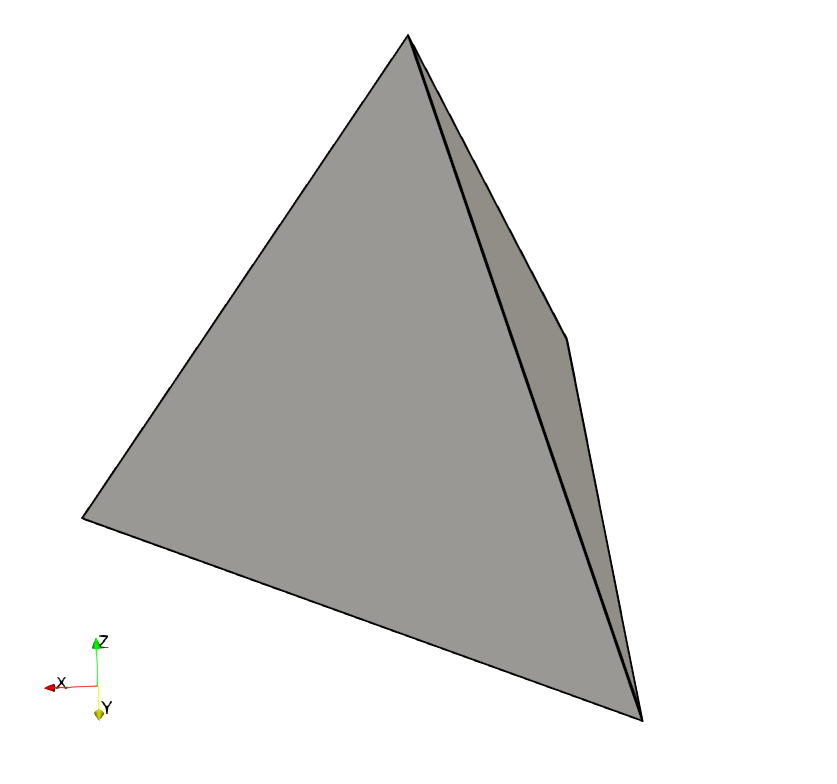
\includegraphics[width=4cm]{python_codes/fieldstone_113/results/test1/tet}
\end{center}

The volume of a regular tetrahedron of edge $l$ is given by:
\[
V=\frac{l^3}{6\sqrt{2}} = \frac{8}{9\sqrt{3}} \simeq 0.5132
\]
and this is what we indeed recover.

\begin{lstlisting}
pt_meas = np.array([0,0,10],dtype=np.float64)
pt_one=np.array([0,0,1],dtype=np.float64)
pt_two=np.array([-np.sqrt(2/9),-np.sqrt(2/3),-1/3],dtype=np.float64)
pt_three=np.array([np.sqrt(8/9),0,-1/3],dtype=np.float64)
pt_four=np.array([-np.sqrt(2/9),np.sqrt(2/3),-1/3],dtype=np.float64)
\end{lstlisting}

\begin{center}
\includegraphics[width=8cm]{python_codes/fieldstone_113/results/test1/g_vector.pdf}
\includegraphics[width=8cm]{python_codes/fieldstone_113/results/test1/g_vector_diff.pdf}\\
\includegraphics[width=8cm]{python_codes/fieldstone_113/results/test1/g_pot.pdf}
\includegraphics[width=8cm]{python_codes/fieldstone_113/results/test1/g_pot_diff.pdf}
\end{center}

%..............................................
\section*{Tetrahedron test 2: the 111-tetrahedron}

It is defined in \textcite{mequ86} (1986) (with a correction by \textcite{camq86} (1986)).

\begin{center}
\includegraphics[width=8cm]{python_codes/fieldstone_113/images/mequ86a}
\end{center}

\begin{lstlisting}
alpha=1.
pt_meas = np.array([2,0.5,0.5],dtype=np.float64)
pt_one=np.array([alpha,alpha,alpha],dtype=np.float64)
pt_two=np.array([alpha,0,0],dtype=np.float64)
pt_three=np.array([0,alpha,0],dtype=np.float64)
pt_four=np.array([0,0,alpha],dtype=np.float64)
\end{lstlisting}


In this case I choose pt1 is node C, pt2 is H, pt3 is F pt 4 is A.
If the cube is a unit cube then the edge length is $\sqrt{2}$ and the volume
\[
V=\frac{l^3}{6\sqrt{2}} = \frac13
\]

\begin{center}
\includegraphics[width=5cm]{python_codes/fieldstone_113/images/tet2}
\end{center}

\textcite{mequ86} state: ``To ensure that the above analysis can be treated
with confidence we have performed numerical calculations of the field components Fx, Fy, and 
Fz using the expressions developed in this paper and
have compared them with those obtained by direct numerical integration'':
\begin{center}
\includegraphics[width=7cm]{python_codes/fieldstone_113/images/mequ86b}\\
{\captionfont Taken from \textcite{mequ86}.}
\end{center}

\begin{center}
\begin{tabular}{lllcc}
\hline
$x$ & $y$ & $z$ & $g_x$ (tet) & $g_x$ (point mass) \\
\hline
\hline
1.25 & 0.5 & 0.5 &  0.566679144260546  & 0.5925925925925926 \\
1.5  & 0.5 & 0.5 &  0.326526930616740  & 0.3333333333333333 \\
1.75 & 0.5 & 0.5 &  0.211222015971550  & 0.2133333333333333 \\
2.0  & 0.5 & 0.5 &  0.147377525744174  & 0.1481481481481481 \\
\hline
\end{tabular}\\
Results obtained with this \stone.
\end{center}

Gravity fields are measured on a line starting at $(1,0.456,0.567)$ and ending at $(5,0.456,0.567)$
\begin{center}
\includegraphics[width=8cm]{python_codes/fieldstone_113/results/test2/g_vector.pdf}
\includegraphics[width=8cm]{python_codes/fieldstone_113/results/test2/g_vector_diff.pdf}\\
\includegraphics[width=8cm]{python_codes/fieldstone_113/results/test2/g_pot.pdf}
\includegraphics[width=8cm]{python_codes/fieldstone_113/results/test2/g_pot_diff.pdf}
\end{center}


%..........................................
\section*{Tetrahedron test 3: the origin tetrahedron}

This is not a regular tetrahedron since $l_{1} \neq l_4 $.

\begin{center}
\includegraphics[width=5cm]{python_codes/fieldstone_113/images/tet3}
\end{center}


\begin{eqnarray}
(x_1,y_1,z_1) &=& (0,0,0) \nn\\
(x_2,y_2,z_2) &=& (1,0,0) \nn\\ 
(x_3,y_3,z_3) &=& (0,1,0) \nn\\
(x_4,y_4,z_4) &=& (0,0,1) \nn
\end{eqnarray}

The gravity fields are measured on a line starting at $(1,1,1)$ and ending at $(3,3,3)$:

\begin{center}
\includegraphics[width=7cm]{python_codes/fieldstone_113/results/test3/g_vector.pdf}
\includegraphics[width=7cm]{python_codes/fieldstone_113/results/test3/g_vector_diff.pdf}\\
\includegraphics[width=7cm]{python_codes/fieldstone_113/results/test3/g_pot.pdf}
\includegraphics[width=7cm]{python_codes/fieldstone_113/results/test3/g_pot_diff.pdf}
\end{center}


%.................................................
\section*{Tetrahedron test 4: cube containing 5 tetrahedra}

{\color{red} to do!}


\newpage
%===============================================================
\section*{Hexahedron: theory}


In what follows $e={\color{purple} 1,2,3,...}$ stands for an edge while $f=A,B,C,...$ stands for a face. 
Each polyhedron face has an outward-pointing face normal vector $\vec{n}_f$
and a face dyad ${\bm F}_f =\vec{n}_f\vec{n}_f $.
Each edge of each face has an outward-pointing edge normal
vector $\vec{n}_{e,f}$ perpendicular to both $\vec{n}_f$ and the edge.
For the edge connecting vertices 1 and 2 shared by faces A and B,
the edge dyad is ${\bm E}_{12}=\vec{n}_A \vec{n}_{12,A}+\vec{n}_B \vec{n}_{21,B}$.

Let $\vec{r}_i$ represent the vector from the variable 
field-point M at location $\vec{r}_M$ to polyhedron vertex $P_i$, 
and let $r_i = ||\vec{r}_i||$ be its length.


For the polyhedron edge connecting
vertices $i$ and $j$ of length $l_{ij}$, the dimensionless per-edge factor $L_e$ is
\[
L_e=L_{ij} = \int_e \frac{1}{r}ds = \int_{P_i}^{P_j} \frac{1}{r} ds 
= \ln \frac{r_i+r_j+l_{ij}}{r_i+r_j-l_{ij}}
\]
For a triangular face $f$ bounded by vertices $i,j,k$ the dimensionless
per-face factor $\omega_f$ is  
\[
\omega_f = 
\iint_{triangle} \frac{\Delta z}{r^3} dS 
= 2 \arctan \frac{\vec{r_i} \cdot (\vec{r}_j \times \vec{r}_k)}{r_ir_jr_k 
+r_i(\vec{r}_j\cdot\vec{r}_k) 
+r_j(\vec{r}_k\cdot\vec{r}_i) 
+r_k(\vec{r}_i\cdot\vec{r}_j) 
}
\]

\begin{center}
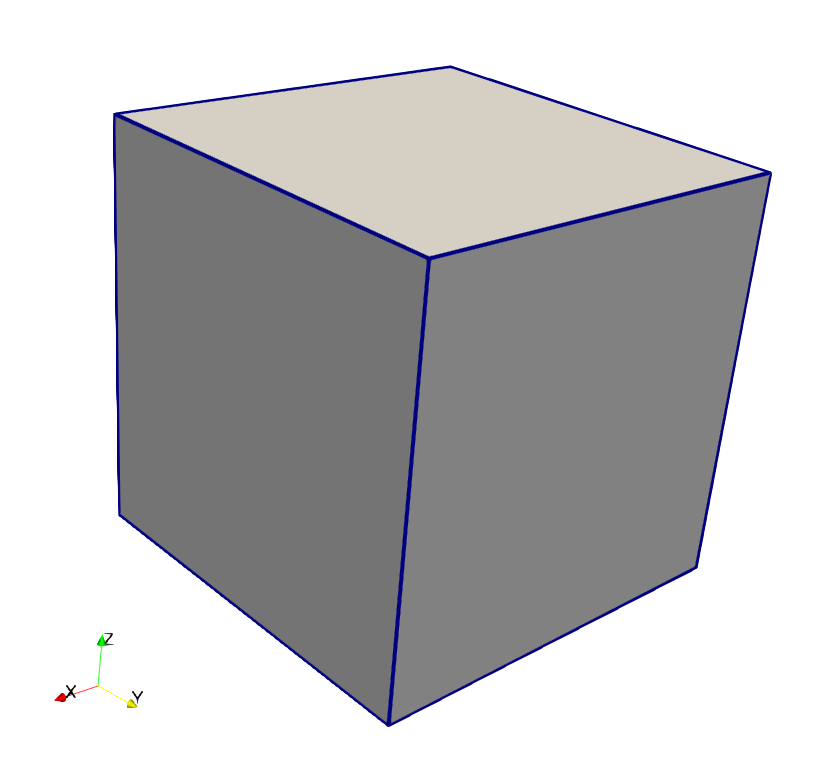
\includegraphics[width=5cm]{python_codes/fieldstone_113/images/hex1}
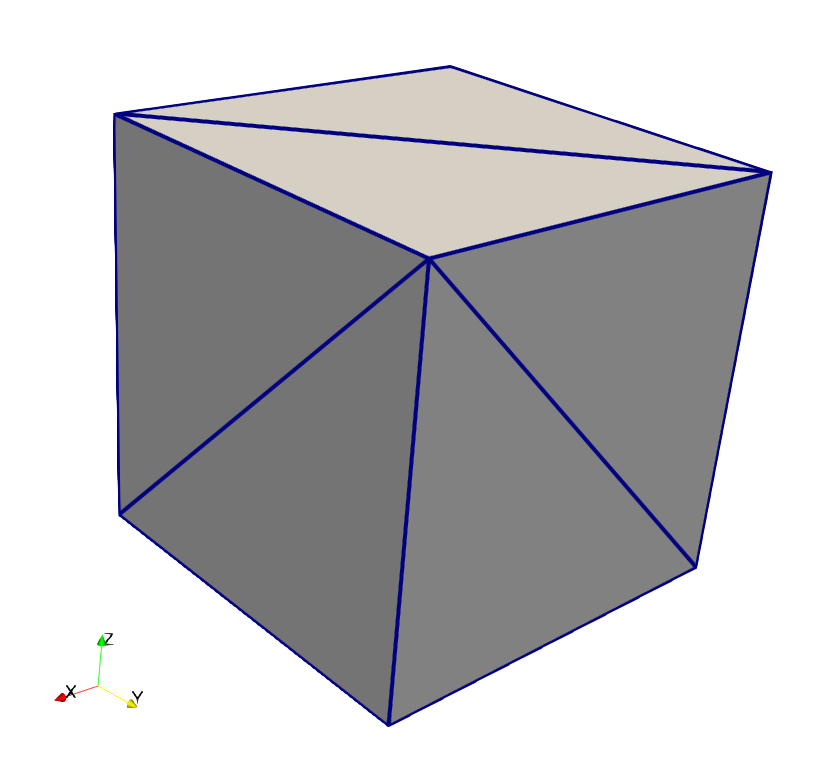
\includegraphics[width=5cm]{python_codes/fieldstone_113/images/hex2}\\
{\captionfont Left: unit cube; Right: triangles making up the visible faces.}
\end{center}

\begin{center}
\includegraphics[width=15cm]{python_codes/fieldstone_113/images/faces/drawing}
\end{center}


When looking at a face from the outside towards the tetrahedron the numbering 
of vertices is counter-clockwise.
\begin{center}
\begin{tabular}{ccccc}
\hline
face & vertices $i,j,k$ & edge \#1 & edge \#2 & edge \#3 \\
\hline\hline
A& 5,1,6 & 5-1 ({\color{purple}9})  & 1-6 ({\color{purple}13})  & 6-5 ({\color{purple}1})  \\
B& 2,6,1 & 2-6 ({\color{purple}10}) & 6-1 ({\color{purple}13})  & 1-2 ({\color{purple}5})  \\
C& 6,2,7 & 6-2 ({\color{purple}10}) & 2-7 ({\color{purple}14})  & 7-6 ({\color{purple}2})  \\
D& 3,7,2 & 3-7 ({\color{purple}11}) & 7-2 ({\color{purple}14})  & 2-3 ({\color{purple}6})  \\
E& 3,4,7 & 3-4 ({\color{purple}7})  & 4-7 ({\color{purple}15})  & 7-3 ({\color{purple}11}) \\
F& 8,7,4 & 8-7 ({\color{purple}3})  & 7-4 ({\color{purple}15})  & 4-8 ({\color{purple}12}) \\
G& 8,4,5 & 8-4 ({\color{purple}12}) & 4-5 ({\color{purple}16})  & 5-8 ({\color{purple}4})  \\
H& 1,5,4 & 1-5 ({\color{purple}9})  & 5-4 ({\color{purple}16})  & 4-1 ({\color{purple}8})  \\
I& 7,8,6 & 7-8 ({\color{purple}3})  & 8-6 ({\color{purple}17})  & 6-7 ({\color{purple}2})  \\
J& 5,6,8 & 5-6 ({\color{purple}1})  & 6-8 ({\color{purple}17})  & 8-5 ({\color{purple}4})  \\
K& 4,3,1 & 4-3 ({\color{purple}7})  & 3-1 ({\color{purple}18})  & 1-4 ({\color{purple}8})  \\
L& 2,1,3 & 2-1 ({\color{purple}5})  & 1-3 ({\color{purple}18})  & 3-2 ({\color{purple}6})  \\
\hline
\end{tabular}
\end{center}


%===============================================================
\section*{Hexahedron: algorithm}

\begin{enumerate}

%.....................................................................................................
\item compute $\vec{l}_{\color{purple}1}$, $\vec{l}_{\color{purple}2}$,etc ... and their norms
$\rightarrow$ \verb|vec_l01|, \verb|vec_l02|, \verb|vec_l03|, \verb|vec_l04|, ... \verb|vec_l18|

\[
\vec{l}_{\color{purple}1} = \vec{l}_{\color{teal}56} = \left(
\begin{array}{c}
x_{\color{teal}6}-x_{\color{teal}5} \\
y_{\color{teal}6}-y_{\color{teal}5} \\
z_{\color{teal}6}-z_{\color{teal}5}
\end{array}
\right)
\qquad
\vec{l}_{\color{purple}2} = \vec{l}_{\color{teal}67} = \left(
\begin{array}{c}
x_{\color{teal}7}-x_{\color{teal}6} \\
y_{\color{teal}7}-y_{\color{teal}6} \\
z_{\color{teal}7}-z_{\color{teal}6}
\end{array}
\right)
\qquad
\textrm{etc...}
\]

{\tiny
\begin{lstlisting}
    vec_l01=np.zeros(3,dtype=np.float64) ; vec_l01 = pt_5-pt_6 ; l01 = LA.norm(vec_l01,2)
    vec_l02=np.zeros(3,dtype=np.float64) ; vec_l02 = pt_6-pt_7 ; l02 = LA.norm(vec_l02,2)
    vec_l03=np.zeros(3,dtype=np.float64) ; vec_l03 = pt_7-pt_8 ; l03 = LA.norm(vec_l03,2)
    ...
    vec_l16=np.zeros(3,dtype=np.float64) ; vec_l16 = pt_4-pt_5 ; l16 = LA.norm(vec_l16,2)
    vec_l17=np.zeros(3,dtype=np.float64) ; vec_l17 = pt_6-pt_8 ; l17 = LA.norm(vec_l17,2)
    vec_l18=np.zeros(3,dtype=np.float64) ; vec_l18 = pt_1-pt_3 ; l18 = LA.norm(vec_l18,2)
\end{lstlisting}
}

%.................................................................................................
\item compute $\vec{r}_{\color{teal} 1,2,3,4,5,6,7,8}$. $\rightarrow$ \verb|vec_r01|, \verb|vec_r02|, \verb|vec_r03|, ... \verb|vec_r08|.
For example:
\[
\vec{r}_{\color{teal}1} = \vec{M1} = \left(
\begin{array}{c}
x_{\color{teal}1}-x_m \\
y_{\color{teal}1}-y_m \\
z_{\color{teal}1}-z_m
\end{array}
\right)
\qquad\qquad
r_{\color{teal}1}= |\vec{r}_{\color{teal}1}|
\]

{\tiny
\begin{lstlisting}
    vec_r01=np.zeros(3,dtype=np.float64) ; vec_r01 = pt_1-pt_M ; r01=LA.norm(vec_r01,2)
    vec_r02=np.zeros(3,dtype=np.float64) ; vec_r02 = pt_2-pt_M ; r02=LA.norm(vec_r02,2)
    vec_r03=np.zeros(3,dtype=np.float64) ; vec_r03 = pt_3-pt_M ; r03=LA.norm(vec_r03,2)
    vec_r04=np.zeros(3,dtype=np.float64) ; vec_r04 = pt_4-pt_M ; r04=LA.norm(vec_r04,2)
    vec_r05=np.zeros(3,dtype=np.float64) ; vec_r05 = pt_5-pt_M ; r05=LA.norm(vec_r05,2)
    vec_r06=np.zeros(3,dtype=np.float64) ; vec_r06 = pt_6-pt_M ; r06=LA.norm(vec_r06,2)
    vec_r07=np.zeros(3,dtype=np.float64) ; vec_r07 = pt_7-pt_M ; r07=LA.norm(vec_r07,2)
    vec_r08=np.zeros(3,dtype=np.float64) ; vec_r08 = pt_8-pt_M ; r08=LA.norm(vec_r08,2)

    r01=LA.norm(vec_r01,2)
    r02=LA.norm(vec_r02,2)
    r03=LA.norm(vec_r03,2)
    r04=LA.norm(vec_r04,2)
    r05=LA.norm(vec_r05,2)
    r06=LA.norm(vec_r06,2)
    r07=LA.norm(vec_r07,2)
    r08=LA.norm(vec_r08,2)
\end{lstlisting}
}


%.................................................................................................
\item compute $\vec{n}_{A,B,C,D,...K,L}$ and coordinates of face centers. 
$\rightarrow$ \verb|vec_nA| , \verb|vec_nB|, \verb|vec_nC|, \verb|vec_nD|, ... \verb|vec_nK|, \verb|vec_nL|

\begin{eqnarray}
\vec{n}_A 
&=& \vec{l}_{\color{teal}51}\times\vec{l}_{\color{teal}56}/
   |\vec{l}_{\color{teal}51}\times\vec{l}_{\color{teal}56}|
= -\vec{l}_{\color{purple}9}\times\vec{l}_{\color{purple}1}/
| -\vec{l}_{\color{purple}9}\times\vec{l}_{\color{purple}1}| 
\nn\\
\vec{n}_B 
&=& \vec{l}_{\color{teal}26}\times\vec{l}_{\color{teal}21}/
   |\vec{l}_{\color{teal}26}\times\vec{l}_{\color{teal}21}|
= \vec{l}_{\color{purple}10}\times-\vec{l}_{\color{purple}5}/
 |\vec{l}_{\color{purple}10}\times-\vec{l}_{\color{purple}5}|  
\nn\\
\vec{n}_C 
&=& \vec{l}_{\color{teal}62}\times\vec{l}_{\color{teal}67}/
   |\vec{l}_{\color{teal}62}\times\vec{l}_{\color{teal}67}|   
= -\vec{l}_{\color{purple}10}\times\vec{l}_{\color{purple}2}/
 |-\vec{l}_{\color{purple}10}\times\vec{l}_{\color{purple}2}| 
\nn  \\
\vec{n}_D 
&=& \vec{l}_{\color{teal}37}\times\vec{l}_{\color{teal}32}/
   |\vec{l}_{\color{teal}37}\times\vec{l}_{\color{teal}32}|   
= \vec{l}_{\color{purple}11}\times-\vec{l}_{\color{purple}6}/
 |\vec{l}_{\color{purple}11}\times-\vec{l}_{\color{purple}6}|
\nn\\
\vec{n}_E
&=& \vec{l}_{\color{teal}34}\times\vec{l}_{\color{teal}37}/
   |\vec{l}_{\color{teal}34}\times\vec{l}_{\color{teal}37}|   
= \vec{l}_{\color{purple}7}\times\vec{l}_{\color{purple}11}/
 |\vec{l}_{\color{purple}7}\times\vec{l}_{\color{purple}11}|
\nn\\
\vec{n}_F
&=& \vec{l}_{\color{teal}87}\times\vec{l}_{\color{teal}84}/
   |\vec{l}_{\color{teal}87}\times\vec{l}_{\color{teal}84}|   
= -\vec{l}_{\color{purple}3}\times-\vec{l}_{\color{purple}12}/
 |-\vec{l}_{\color{purple}3}\times-\vec{l}_{\color{purple}12}|
\nn\\
\vec{n}_G
&=& \vec{l}_{\color{teal}84}\times\vec{l}_{\color{teal}85}/
   |\vec{l}_{\color{teal}84}\times\vec{l}_{\color{teal}85}|   
= -\vec{l}_{\color{purple}12}\times\vec{l}_{\color{purple}4}/
 |-\vec{l}_{\color{purple}12}\times\vec{l}_{\color{purple}4}|
\nn\\
\vec{n}_H
&=& \vec{l}_{\color{teal}15}\times\vec{l}_{\color{teal}14}/
   |\vec{l}_{\color{teal}14}\times\vec{l}_{\color{teal}14}|   
= \vec{l}_{\color{purple}9}\times-\vec{l}_{\color{purple}8}/
 |\vec{l}_{\color{purple}9}\times-\vec{l}_{\color{purple}8}|
\nn\\
\vec{n}_I
&=& \vec{l}_{\color{teal}78}\times\vec{l}_{\color{teal}76}/
   |\vec{l}_{\color{teal}78}\times\vec{l}_{\color{teal}76}|   
= \vec{l}_{\color{purple}3}\times-\vec{l}_{\color{purple}2}/
 |\vec{l}_{\color{purple}3}\times-\vec{l}_{\color{purple}2}|
\nn\\
\vec{n}_J
&=& \vec{l}_{\color{teal}56}\times\vec{l}_{\color{teal}58}/
   |\vec{l}_{\color{teal}56}\times\vec{l}_{\color{teal}58}|   
= \vec{l}_{\color{purple}1}\times-\vec{l}_{\color{purple}4}/
 |\vec{l}_{\color{purple}1}\times-\vec{l}_{\color{purple}4}|
\nn\\
\vec{n}_K
&=& \vec{l}_{\color{teal}43}\times\vec{l}_{\color{teal}41}/
   |\vec{l}_{\color{teal}43}\times\vec{l}_{\color{teal}41}|   
= -\vec{l}_{\color{purple}7}\times\vec{l}_{\color{purple}8}/
 |-\vec{l}_{\color{purple}7}\times\vec{l}_{\color{purple}8}|
\nn\\
\vec{n}_L
&=& \vec{l}_{\color{teal}21}\times\vec{l}_{\color{teal}23}/
   |\vec{l}_{\color{teal}21}\times\vec{l}_{\color{teal}23}|   
= -\vec{l}_{\color{purple}5}\times\vec{l}_{\color{purple}6}/
 |-\vec{l}_{\color{purple}5}\times\vec{l}_{\color{purple}6}|
\nn
\end{eqnarray}

{\tiny
\begin{lstlisting}
pt_midA=np.zeros(3,dtype=np.float64) ; pt_midA = (pt_1+pt_6+pt_5)/3
pt_midB=np.zeros(3,dtype=np.float64) ; pt_midB = (pt_1+pt_2+pt_6)/3
pt_midC=np.zeros(3,dtype=np.float64) ; pt_midC = (pt_2+pt_7+pt_6)/3 
...
pt_midJ=np.zeros(3,dtype=np.float64) ; pt_midJ = (pt_8+pt_5+pt_6)/3
pt_midK=np.zeros(3,dtype=np.float64) ; pt_midK = (pt_3+pt_1+pt_4)/3
pt_midL=np.zeros(3,dtype=np.float64) ; pt_midL = (pt_3+pt_2+pt_1)/3

vec_nA=np.cross( vec_l13, vec_l09) ; vec_nA/=LA.norm(vec_nA,2)
vec_nB=np.cross( vec_l10,-vec_l05) ; vec_nB/=LA.norm(vec_nB,2)
vec_nC=np.cross(-vec_l10, vec_l02) ; vec_nC/=LA.norm(vec_nC,2)
...
vec_nJ=np.cross( vec_l01,-vec_l04) ; vec_nJ/=LA.norm(vec_nJ,2)
vec_nK=np.cross(-vec_l07, vec_l08) ; vec_nK/=LA.norm(vec_nK,2)
vec_nL=np.cross(-vec_l05, vec_l06) ; vec_nL/=LA.norm(vec_nL,2)
\end{lstlisting}
}

%.....................................................................................
\item compute ${\bm F}_{A,B,C,D}$. 
$\rightarrow$ \verb|mat_FaceA| , \verb|mat_FaceB|, \verb|mat_FaceC|, 
\verb|mat_FaceD|, ... \verb|mat_FaceL|

\begin{eqnarray}
{\bm F}_A &=& \vec{n}_A\vec{n}_A \nn\\
{\bm F}_B &=& \vec{n}_B\vec{n}_B \nn\\
{\bm F}_C &=& \vec{n}_C\vec{n}_C \nn\\
... \nn\\
{\bm F}_K &=& \vec{n}_K\vec{n}_K \nn\\
{\bm F}_L &=& \vec{n}_L\vec{n}_L \nn
\end{eqnarray}

{\tiny
\begin{lstlisting}
mat_FA=np.zeros((3,3),dtype=np.float64) ; mat_FA=np.outer(vec_nA,vec_nA)
mat_FB=np.zeros((3,3),dtype=np.float64) ; mat_FB=np.outer(vec_nB,vec_nB)
mat_FC=np.zeros((3,3),dtype=np.float64) ; mat_FC=np.outer(vec_nC,vec_nC)
...
mat_FJ=np.zeros((3,3),dtype=np.float64) ; mat_FJ=np.outer(vec_nJ,vec_nJ)
mat_FK=np.zeros((3,3),dtype=np.float64) ; mat_FK=np.outer(vec_nK,vec_nK)
mat_FL=np.zeros((3,3),dtype=np.float64) ; mat_FL=np.outer(vec_nL,vec_nL)
\end{lstlisting}
}

%............................................................................................
\item compute $\omega_{A,B,C,D}$. $\rightarrow$ \verb|wA|, \verb|wB|, \verb|wC|, \verb|wD|, ... \verb|wK|, \verb|wL|.
In what follows $r_i=|\vec{r}_i|$.


\begin{eqnarray}
\omega_A &=& 
2 \arctan \frac{\vec{r_{\color{teal}5}} \cdot (\vec{r}_{\color{teal}1} \times \vec{r}_{\color{teal}6})}
{{r}_{\color{teal}5}{r}_{\color{teal}1}{r}_{\color{teal}6} 
+{r}_{\color{teal}1}(\vec{r}_{\color{teal}6}\cdot\vec{r}_{\color{teal}5}) 
+{r}_{\color{teal}6}(\vec{r}_{\color{teal}5}\cdot\vec{r}_{\color{teal}1}) 
+{r}_{\color{teal}5}(\vec{r}_{\color{teal}1}\cdot\vec{r}_{\color{teal}6})  }  
\qquad A=\{{\color{teal}5,1,6}\}=\{ {\color{purple} 9,13,1} \}
\nn\\
\omega_B &=& 
2 \arctan \frac{\vec{r_{\color{teal}2}} \cdot (\vec{r}_{\color{teal}6} \times \vec{r}_{\color{teal}1})}
{{r}_{\color{teal}2}{r}_{\color{teal}6}{r}_{\color{teal}1} 
+{r}_{\color{teal}1}(\vec{r}_{\color{teal}2}\cdot\vec{r}_{\color{teal}6}) 
+{r}_{\color{teal}2}(\vec{r}_{\color{teal}6}\cdot\vec{r}_{\color{teal}1}) 
+{r}_{\color{teal}6}(\vec{r}_{\color{teal}1}\cdot\vec{r}_{\color{teal}2})  }  
\qquad B=\{ {\color{teal}2,6,1} \}=\{ {\color{purple} 10,13,5} \}
\nn\\
\omega_C &=& 
2 \arctan \frac{\vec{r_{\color{teal}6}} \cdot (\vec{r}_{\color{teal}2} \times \vec{r}_{\color{teal}7})}
{{r}_{\color{teal}6}{r}_{\color{teal}2}{r}_{\color{teal}7} 
+{r}_{\color{teal}2}(\vec{r}_{\color{teal}7}\cdot\vec{r}_{\color{teal}6}) 
+{r}_{\color{teal}7}(\vec{r}_{\color{teal}6}\cdot\vec{r}_{\color{teal}2}) 
+{r}_{\color{teal}6}(\vec{r}_{\color{teal}2}\cdot\vec{r}_{\color{teal}7})  }  
\qquad C=\{ {\color{teal}6,2,7} \}=\{ {\color{purple} 10,14,2} \}
\nn\\
\omega_D &=& 
2 \arctan \frac{\vec{r_{\color{teal}3}} \cdot (\vec{r}_{\color{teal}7} \times \vec{r}_{\color{teal}2})}
{{r}_{\color{teal}3}{r}_{\color{teal}7}{r}_{\color{teal}2} 
+{r}_{\color{teal}2}(\vec{r}_{\color{teal}3}\cdot\vec{r}_{\color{teal}7}) 
+{r}_{\color{teal}3}(\vec{r}_{\color{teal}7}\cdot\vec{r}_{\color{teal}2}) 
+{r}_{\color{teal}7}(\vec{r}_{\color{teal}2}\cdot\vec{r}_{\color{teal}3})  }  
\qquad D=\{ {\color{teal}3,7,2} \}=\{ {\color{purple} 11,14,6} \}
\nn\\
\omega_E &=& 
2 \arctan \frac{\vec{r_{\color{teal}3}} \cdot (\vec{r}_{\color{teal}4} \times \vec{r}_{\color{teal}7})}
{{r}_{\color{teal}3}{r}_{\color{teal}4}{r}_{\color{teal}7} 
+{r}_{\color{teal}1}(\vec{r}_{\color{teal}6}\cdot\vec{r}_{\color{teal}5}) 
+{r}_{\color{teal}6}(\vec{r}_{\color{teal}5}\cdot\vec{r}_{\color{teal}1}) 
+{r}_{\color{teal}5}(\vec{r}_{\color{teal}1}\cdot\vec{r}_{\color{teal}6})  }  
\qquad E=\{ {\color{teal} 3,4,7} \}=\{ {\color{purple} 7,15,11} \}
\nn\\
\omega_F &=& 
2 \arctan \frac{\vec{r_{\color{teal}8}} \cdot (\vec{r}_{\color{teal}7} \times \vec{r}_{\color{teal}4})}
{{r}_{\color{teal}8}{r}_{\color{teal}7}{r}_{\color{teal}4} 
+{r}_{\color{teal}7}(\vec{r}_{\color{teal}4}\cdot\vec{r}_{\color{teal}8}) 
+{r}_{\color{teal}4}(\vec{r}_{\color{teal}8}\cdot\vec{r}_{\color{teal}7}) 
+{r}_{\color{teal}8}(\vec{r}_{\color{teal}7}\cdot\vec{r}_{\color{teal}4})  }  
\qquad F=\{ {\color{teal} 8,7,4} \}=\{ {\color{purple} 3,15,12} \}
\nn\\
\omega_G &=& 
2 \arctan \frac{\vec{r_{\color{teal}8}} \cdot (\vec{r}_{\color{teal}4} \times \vec{r}_{\color{teal}5})}
{{r}_{\color{teal}8}{r}_{\color{teal}4}{r}_{\color{teal}5} 
+{r}_{\color{teal}4}(\vec{r}_{\color{teal}5}\cdot\vec{r}_{\color{teal}8}) 
+{r}_{\color{teal}5}(\vec{r}_{\color{teal}8}\cdot\vec{r}_{\color{teal}4}) 
+{r}_{\color{teal}8}(\vec{r}_{\color{teal}4}\cdot\vec{r}_{\color{teal}5})  }  
\qquad G=\{ {\color{teal}8,4,5} \}=\{ {\color{purple} 12,16,4} \}
\nn\\
\omega_H &=& 
2 \arctan \frac{\vec{r_{\color{teal}1}} \cdot (\vec{r}_{\color{teal}5} \times \vec{r}_{\color{teal}4})}
{{r}_{\color{teal}1}{r}_{\color{teal}5}{r}_{\color{teal}4} 
+{r}_{\color{teal}4}(\vec{r}_{\color{teal}1}\cdot\vec{r}_{\color{teal}5}) 
+{r}_{\color{teal}1}(\vec{r}_{\color{teal}5}\cdot\vec{r}_{\color{teal}4}) 
+{r}_{\color{teal}5}(\vec{r}_{\color{teal}4}\cdot\vec{r}_{\color{teal}1})  }  
\qquad H=\{ {\color{teal}1,5,4} \}=\{ {\color{purple} 9,16,8} \}
\nn\\
\omega_I &=& 
2 \arctan \frac{\vec{r_{\color{teal}7}} \cdot (\vec{r}_{\color{teal}8} \times \vec{r}_{\color{teal}6})}
{{r}_{\color{teal}7}{r}_{\color{teal}8}{r}_{\color{teal}6} 
+{r}_{\color{teal}8}(\vec{r}_{\color{teal}6}\cdot\vec{r}_{\color{teal}7}) 
+{r}_{\color{teal}6}(\vec{r}_{\color{teal}7}\cdot\vec{r}_{\color{teal}8}) 
+{r}_{\color{teal}7}(\vec{r}_{\color{teal}8}\cdot\vec{r}_{\color{teal}6})  }  
\qquad I=\{ {\color{teal}7,8,6}\}=\{ {\color{purple} 3,17,2} \}
\nn\\
\omega_J &=& 
2 \arctan \frac{\vec{r_{\color{teal}5}} \cdot (\vec{r}_{\color{teal}6} \times \vec{r}_{\color{teal}8})}
{{r}_{\color{teal}5}{r}_{\color{teal}6}{r}_{\color{teal}8} 
+{r}_{\color{teal}8}(\vec{r}_{\color{teal}5}\cdot\vec{r}_{\color{teal}6}) 
+{r}_{\color{teal}5}(\vec{r}_{\color{teal}6}\cdot\vec{r}_{\color{teal}8}) 
+{r}_{\color{teal}6}(\vec{r}_{\color{teal}8}\cdot\vec{r}_{\color{teal}5})  }  
\qquad J=\{ {\color{teal}5,6,8}\}=\{ {\color{purple} 1,17,4} \}
\nn\\
\omega_K &=& 
2 \arctan \frac{\vec{r_{\color{teal}4}} \cdot (\vec{r}_{\color{teal}3} \times \vec{r}_{\color{teal}1})}
{{r}_{\color{teal}4}{r}_{\color{teal}3}{r}_{\color{teal}1} 
+{r}_{\color{teal}3}(\vec{r}_{\color{teal}1}\cdot\vec{r}_{\color{teal}4}) 
+{r}_{\color{teal}1}(\vec{r}_{\color{teal}4}\cdot\vec{r}_{\color{teal}3}) 
+{r}_{\color{teal}4}(\vec{r}_{\color{teal}3}\cdot\vec{r}_{\color{teal}1})  }  
\qquad K=\{{\color{teal}4,3,1}\}=\{ {\color{purple} 7,18,8} \}
\nn\\
\omega_L &=& 
2 \arctan \frac{\vec{r_{\color{teal}2}} \cdot (\vec{r}_{\color{teal}1} \times \vec{r}_{\color{teal}3})}
{{r}_{\color{teal}2}{r}_{\color{teal}1}{r}_{\color{teal}3} 
+{r}_{\color{teal}3}(\vec{r}_{\color{teal}2}\cdot\vec{r}_{\color{teal}1}) 
+{r}_{\color{teal}2}(\vec{r}_{\color{teal}1}\cdot\vec{r}_{\color{teal}3}) 
+{r}_{\color{teal}1}(\vec{r}_{\color{teal}3}\cdot\vec{r}_{\color{teal}2})  }  
\qquad L=\{ {\color{teal}2,1,3}\}=\{ {\color{purple} 5,18,6} \}
\nn
\end{eqnarray}



{\tiny
\begin{lstlisting}
# A: 516
num=np.dot(vec_r05,np.cross(vec_r01,vec_r06))
denom=(r05*r01*r06+r05*np.dot(vec_r01,vec_r06)
      +r01*np.dot(vec_r06,vec_r05)
      +r06*np.dot(vec_r05,vec_r01))
wA=2*np.arctan2(num,denom)

# B: 261
num=np.dot(vec_r02,np.cross(vec_r06,vec_r01))
denom=(r02*r06*r01+r02*np.dot(vec_r06,vec_r01)
      +r06*np.dot(vec_r01,vec_r02)
      +r01*np.dot(vec_r02,vec_r06))
wB=2*np.arctan2(num,denom)

# C: 627
num=np.dot(vec_r06,np.cross(vec_r02,vec_r07))
denom=(r06*r02*r07+r06*np.dot(vec_r02,vec_r07)
      +r02*np.dot(vec_r07,vec_r06)
      +r07*np.dot(vec_r06,vec_r02))
wC=2*np.arctan2(num,denom)

...
\end{lstlisting}
}




%..........................................................................................step6
\item compute $\vec{r}_{A}$, $\vec{r}_{B}$, $\vec{r}_{C}$, $\vec{r}_{D}$.
As explained in the caption of their Figure~3, ``vector $\vec{r}_f$
extends from the field point $M$ to any point in the face plane''.
$\rightarrow$ \verb|vec_rA|, \verb|vec_rB|, \verb|vec_rC|, \verb|vec_rD|, ... \verb|ver_rL|

{\tiny
\begin{lstlisting}
    vec_rA = pt_midA-pt_M
    vec_rB = pt_midB-pt_M
    vec_rC = pt_midC-pt_M
    vec_rD = pt_midD-pt_M
    vec_rE = pt_midE-pt_M
    vec_rF = pt_midF-pt_M
    vec_rG = pt_midG-pt_M
    vec_rH = pt_midH-pt_M
    vec_rI = pt_midI-pt_M
    vec_rJ = pt_midJ-pt_M
    vec_rK = pt_midK-pt_M
    vec_rL = pt_midL-pt_M
\end{lstlisting}
}




%...........................................................................................step7
\item compute $\vec{g}_f$ by means of % Eq.~\eqref{eq:tetra:gf}

\[
\vec{g}_f
= {\cal G} \rho_0 \sum_f \omega_f {\bm F}_f\cdot \vec{r}_f 
= {\cal G} \rho_0 \left(
\omega_A {\bm F}_A\cdot \vec{r}_A +
\omega_B {\bm F}_B\cdot \vec{r}_B +
\omega_C {\bm F}_C\cdot \vec{r}_C +
\omega_D {\bm F}_D\cdot \vec{r}_D +
...+
\omega_L {\bm F}_L \cdot \vec{r}_L
\right)
\]

{\tiny
\begin{lstlisting}
    vec_gf=np.zeros(3,dtype=np.float64)
    vec_gf=wA*np.dot(mat_FA,vec_rA) +\
           wB*np.dot(mat_FB,vec_rB) +\
           wC*np.dot(mat_FC,vec_rC) +\
           wD*np.dot(mat_FD,vec_rD) +\
           wE*np.dot(mat_FE,vec_rE) +\
           wF*np.dot(mat_FF,vec_rF) +\
           wG*np.dot(mat_FG,vec_rG) +\
           wH*np.dot(mat_FH,vec_rH) +\
           wI*np.dot(mat_FI,vec_rI) +\
           wJ*np.dot(mat_FJ,vec_rJ) +\
           wK*np.dot(mat_FK,vec_rK) +\
           wL*np.dot(mat_FL,vec_rL)
    vec_gf*=Ggrav*rho0
\end{lstlisting}
}


%.........................................................................................step8
\item compute $\vec{n}_{e,f}$ for each edge of each face (12 triangles*3=36 vectors!)
$\rightarrow$ \verb|vec_nA12|, \verb|vec_nA23|, \verb|vec_nA13|, \verb|vec_nB13|, etc ...

{\tiny
\begin{lstlisting}
    vec_nA12 = compute_face_edge_normal(vec_nA,pt_1,pt_2,pt_midA,'faceA_n12')
    vec_nA23 = compute_face_edge_normal(vec_nA,pt_2,pt_3,pt_midA,'faceA_n23')
    vec_nA13 = compute_face_edge_normal(vec_nA,pt_3,pt_1,pt_midA,'faceA_n31')
\end{lstlisting}
}




%.........................................................................................step9
\item compute ${\bm E}_{\color{purple} 1,2,3,4,5,6,...18}$.
$\rightarrow$ \verb|mat_E12, mat_E13, mat_E14, mat_E23, mat_E24, mat_E34|.
For the edge connecting vertices 1 and 2 shared by faces A and B,
the edge dyad is ${\bm E}_{12}=\vec{n}_A \vec{n}_{12,A}+\vec{n}_B \vec{n}_{21,B}$.


\begin{center}
\begin{tabular}{ccccc}
\hline
edge & vertices & belongs to \\
{\color{purple}1}  & 5,6 & J,A\\
{\color{purple}2}  & 6,7 & I,C\\
{\color{purple}3}  & 7,8 & I,F\\
{\color{purple}4}  & 8,5 & J,G\\
{\color{purple}5}  & 1,2 & B,L\\
{\color{purple}6}  & 2,3 & D,L\\
{\color{purple}7}  & 3,4 & E,K\\
{\color{purple}8}  & 4,1 & H,K\\
{\color{purple}9}  & 1,5 & H,A\\
{\color{purple}10} & 2,6 & B,C \\
{\color{purple}11} & 3,7 & D,E\\
{\color{purple}12} & 4,8 & F,G\\
{\color{purple}13} & 1,6 & A,B\\
{\color{purple}14} & 2,7 & C,D\\
{\color{purple}15} & 4,7 & E,F\\
{\color{purple}16} & 4,5 & G,H\\
{\color{purple}17} & 6,8 & J,I\\
{\color{purple}18} & 1,3 & L,K\\
\hline
\end{tabular}
\end{center}
The first letter is the face left of the arrow, the second letter is the face right of the arrow, 
when going along the arrow.

\begin{center}
\begin{tikzpicture}
%\draw[step=0.5cm,gray,very thin] (0,0) grid (12,8.5); 
\draw[thick] (0.6,2.8) -- (3,5.6)--(6.7,6.9);
\draw[thick] (3,5.6)  -- (8.1,3.2) ;
\draw[thick] (5.9,0.4) -- (8.1,3.2) -- (11.1,4.2);
\node[] at (9,4.5) {face A}; 
\node[] at (4.5,2) {face B}; 
\draw[thick,->] (2.4,3.5)--(0.5,5); 
\node[] at (0.5,5.25) {$\vec{n}_B$};
\draw[] (2.2,3.65) -- (2.38,3.85) --(2.58,3.66);
\draw[thick,->] (5.5,5.7)--(5.2,8.1); 
\node[] at (5.6,8) {$\vec{n}_A$};
\draw[] (5.45,6) --(5.7,6.075) --(5.75,5.8);
\node[] at (2.7,5.7) {1};
\node[] at (8.2,2.85) {2};
\draw[black,fill=teal] (3,5.6) circle (3pt);
\draw[black,fill=teal] (8.1,3.2) circle (3pt);
\node[] at (8,5.8) {$\vec{n}_{21,B}$};
\draw[thick,->] (6.5,4)--(7.75,5.6); 
\node[] at (4,3) {$\vec{n}_{12,A}$};
\draw[thick,->] (6.5,4)--(4.1,3.2); 
\node[rotate=-25] at (5,5) {common edge};
\end{tikzpicture}\\
{\captionfont Figure made after Fig.~7 from \textcite{wesc97}.}
\end{center}


\begin{eqnarray}
{\bm E}_{\color{purple}1} ={\bm E}_{\color{teal}56}
&=&\vec{n}_A \vec{n}_{{\color{teal}12},A} 
+  \vec{n}_J \vec{n}_{{\color{teal}21},J} \nn\\
{\bm E}_{\color{purple}2} ={\bm E}_{\color{teal}67}
&=&\vec{n}_I \vec{n}_{{\color{teal}13},I} 
+  \vec{n}_C \vec{n}_{{\color{teal}13},C} \nn\\
{\bm E}_{\color{purple}3} ={\bm E}_{\color{teal}78}
&=&\vec{n}_F \vec{n}_{{\color{teal}14},F}
+  \vec{n}_I \vec{n}_{{\color{teal}14},I} \nn\\
{\bm E}_{\color{purple}4} ={\bm E}_{\color{teal}85}
&=&\vec{n}_J \vec{n}_{{\color{teal}23},J}
+  \vec{n}_G \vec{n}_{{\color{teal}23},G} \nn\\
{\bm E}_{\color{purple}5} ={\bm E}_{\color{teal}12}
&=&\vec{n}_B \vec{n}_{{\color{teal}24},B} 
+  \vec{n}_L \vec{n}_{{\color{teal}24},L} \nn\\  
{\bm E}_{\color{purple}6} ={\bm E}_{\color{teal}23}
&=&\vec{n}_L \vec{n}_{{\color{teal}34},L} 
+  \vec{n}_D \vec{n}_{{\color{teal}34},D} \nn\\
{\bm E}_{\color{purple}7} ={\bm E}_{\color{teal}34}  
&=&\vec{n}_E \vec{n}_{{\color{teal}34},E} 
+  \vec{n}_K \vec{n}_{{\color{teal}34},K} \nn\\
{\bm E}_{\color{purple}8} ={\bm E}_{\color{teal}41}  
&=&\vec{n}_H \vec{n}_{{\color{teal}34},H} 
+  \vec{n}_K \vec{n}_{{\color{teal}34},K} \nn\\
{\bm E}_{\color{purple}9} ={\bm E}_{\color{teal}15}  
&=&\vec{n}_A \vec{n}_{{\color{teal}34},A} 
+  \vec{n}_H \vec{n}_{{\color{teal}34},H} \nn\\
{\bm E}_{\color{purple}10} ={\bm E}_{\color{teal}26} 
&=&\vec{n}_B \vec{n}_{{\color{teal}34},B} 
+  \vec{n}_C \vec{n}_{{\color{teal}34},C} \nn\\
{\bm E}_{\color{purple}11} ={\bm E}_{\color{teal}37} 
&=&\vec{n}_D \vec{n}_{{\color{teal}34},D} 
+  \vec{n}_E \vec{n}_{{\color{teal}34},E} \nn\\
{\bm E}_{\color{purple}12} ={\bm E}_{\color{teal}48} 
&=&\vec{n}_F \vec{n}_{{\color{teal}34},F} 
+  \vec{n}_G \vec{n}_{{\color{teal}34},G} \nn\\
{\bm E}_{\color{purple}13} ={\bm E}_{\color{teal}16}   
&=&\vec{n}_A \vec{n}_{{\color{teal}34},A} 
+  \vec{n}_B \vec{n}_{{\color{teal}34},B} \nn\\
{\bm E}_{\color{purple}14} ={\bm E}_{\color{teal}27}   
&=&\vec{n}_C \vec{n}_{{\color{teal}34},C} 
+  \vec{n}_D \vec{n}_{{\color{teal}34},D} \nn\\
{\bm E}_{\color{purple}15} ={\bm E}_{\color{teal}47}   
&=&\vec{n}_E \vec{n}_{{\color{teal}47},E} 
+  \vec{n}_F \vec{n}_{{\color{teal}74},F} \nn\\
{\bm E}_{\color{purple}16} ={\bm E}_{\color{teal}45}   
&=&\vec{n}_G \vec{n}_{{\color{teal}45},G} 
+  \vec{n}_H \vec{n}_{{\color{teal}54},H} \nn\\
{\bm E}_{\color{purple}17} ={\bm E}_{\color{teal}68}   
&=&\vec{n}_I \vec{n}_{{\color{teal}68},I} 
+  \vec{n}_J \vec{n}_{{\color{teal}86},J} \nn\\
{\bm E}_{\color{purple}18} ={\bm E}_{\color{teal}13} 
&=&\vec{n}_K \vec{n}_{{\color{teal}13},K} 
+  \vec{n}_L \vec{n}_{{\color{teal}31},L} \nn
\end{eqnarray}

{\tiny
\begin{lstlisting}
mat_E56=np.outer(vec_nJ,vec_nJ56)+np.outer(vec_nA,vec_nA65) #edge 5-6 ( 1) belongs to J & A
mat_E67=np.outer(vec_nI,vec_nI67)+np.outer(vec_nC,vec_nC76) #edge 6-7 ( 2) belongs to I & C
mat_E78=np.outer(vec_nI,vec_nI78)+np.outer(vec_nF,vec_nF87) #edge 7-8 ( 3) belongs to I & F
mat_E85=np.outer(vec_nJ,vec_nJ85)+np.outer(vec_nG,vec_nG58) #edge 8-5 ( 4) belongs to J & G
mat_E12=np.outer(vec_nB,vec_nB12)+np.outer(vec_nL,vec_nL21) #edge 1-2 ( 5) belongs to B & L
mat_E23=np.outer(vec_nD,vec_nD23)+np.outer(vec_nL,vec_nL32) #edge 2-3 ( 6) belongs to D & L
mat_E34=np.outer(vec_nE,vec_nE34)+np.outer(vec_nK,vec_nK43) #edge 3-4 ( 7) belongs to E & K 
mat_E41=np.outer(vec_nH,vec_nH41)+np.outer(vec_nK,vec_nK14) #edge 4-1 ( 8) belongs to H & K
mat_E15=np.outer(vec_nH,vec_nH15)+np.outer(vec_nA,vec_nA51) #edge 1-5 ( 9) belongs to H & A
mat_E26=np.outer(vec_nB,vec_nB26)+np.outer(vec_nC,vec_nC62) #edge 2-6 (10) belongs to B & C
mat_E37=np.outer(vec_nD,vec_nD37)+np.outer(vec_nE,vec_nE73) #edge 3-7 (11) belongs to D & E
mat_E48=np.outer(vec_nF,vec_nF48)+np.outer(vec_nG,vec_nG84) #edge 4-8 (12) belongs to F & G
mat_E16=np.outer(vec_nA,vec_nA16)+np.outer(vec_nB,vec_nB61) #edge 1-6 (13) belongs to A & B
mat_E27=np.outer(vec_nC,vec_nC27)+np.outer(vec_nD,vec_nD72) #edge 2-7 (14) belongs to C & D
mat_E47=np.outer(vec_nE,vec_nE47)+np.outer(vec_nF,vec_nF74) #edge 4-7 (15) belongs to E & F
mat_E45=np.outer(vec_nG,vec_nG45)+np.outer(vec_nH,vec_nH54) #edge 4-5 (16) belongs to G & H
mat_E68=np.outer(vec_nJ,vec_nJ68)+np.outer(vec_nI,vec_nI86) #edge 6-8 (17) belongs to J & I
mat_E13=np.outer(vec_nL,vec_nL13)+np.outer(vec_nK,vec_nK31) #edge 1-3 (18) belongs to L & K
\end{lstlisting}
}


%..................................................................................... step 10
\item compute $L_{\color{purple}1,2,3,4,5,6}$ $\rightarrow$ \verb|L01|, \verb|L02|, \verb|L03|, ... 
\begin{eqnarray}
L_{\color{purple}1} = L_{\color{teal}56} 
&=& \ln \frac{r_{\color{teal}5}+r_{\color{teal}6}+l_{\color{purple}1}}
             {r_{\color{teal}5}+r_{\color{teal}6}-l_{\color{purple}1}} 
\nn\\
L_{\color{purple}2} = L_{\color{teal}67} 
&=& \ln \frac{r_{\color{teal}6}+r_{\color{teal}7}+l_{\color{purple}2}}
             {r_{\color{teal}6}+r_{\color{teal}7}-l_{\color{purple}2}} 
\nn\\
L_{\color{purple}3} = L_{\color{teal}78} 
&=& \ln \frac{r_{\color{teal}7}+r_{\color{teal}8}+l_{\color{purple}3}}
             {r_{\color{teal}7}+r_{\color{teal}8}-l_{\color{purple}3}} 
\nn\\
L_{\color{purple}4} = L_{\color{teal}85} 
&=& \ln \frac{r_{\color{teal}8}+r_{\color{teal}5}+l_{\color{purple}4}}
             {r_{\color{teal}8}+r_{\color{teal}5}-l_{\color{purple}4}} 
\nn\\
L_{\color{purple}5} = L_{\color{teal}12} 
&=& \ln \frac{r_{\color{teal}1}+r_{\color{teal}2}+l_{\color{purple}5}}
             {r_{\color{teal}1}+r_{\color{teal}2}-l_{\color{purple}5}} 
\nn\\
L_{\color{purple}6} = L_{\color{teal}23} 
&=& \ln \frac{r_{\color{teal}2}+r_{\color{teal}3}+l_{\color{purple}6}}
             {r_{\color{teal}2}+r_{\color{teal}3}-l_{\color{purple}6}} 
\nn\\
L_{\color{purple}7} = L_{\color{teal}34} 
&=& \ln \frac{r_{\color{teal}3}+r_{\color{teal}4}+l_{\color{purple}7}}
             {r_{\color{teal}3}+r_{\color{teal}4}-l_{\color{purple}7}} 
\nn\\
L_{\color{purple}8} = L_{\color{teal}41} 
&=& \ln \frac{r_{\color{teal}4}+r_{\color{teal}3}+l_{\color{purple}8}}
             {r_{\color{teal}4}+r_{\color{teal}3}-l_{\color{purple}8}} 
\nn\\
L_{\color{purple}9} = L_{\color{teal}15} 
&=& \ln \frac{r_{\color{teal}1}+r_{\color{teal}5}+l_{\color{purple}9}}
             {r_{\color{teal}1}+r_{\color{teal}5}-l_{\color{purple}9}} 
\nn\\
L_{\color{purple}10} = L_{\color{teal}26} 
&=& \ln \frac{r_{\color{teal}2}+r_{\color{teal}6}+l_{\color{purple}10}}
             {r_{\color{teal}2}+r_{\color{teal}6}-l_{\color{purple}10}} 
\nn\\
L_{\color{purple}11} = L_{\color{teal}37} 
&=& \ln \frac{r_{\color{teal}3}+r_{\color{teal}7}+l_{\color{purple}11}}
             {r_{\color{teal}3}+r_{\color{teal}7}-l_{\color{purple}11}} 
\nn\\
L_{\color{purple}12} = L_{\color{teal}48} 
&=& \ln \frac{r_{\color{teal}4}+r_{\color{teal}8}+l_{\color{purple}12}}
             {r_{\color{teal}4}+r_{\color{teal}8}-l_{\color{purple}12}} 
\nn\\
L_{\color{purple}13} = L_{\color{teal}16} 
&=& \ln \frac{r_{\color{teal}1}+r_{\color{teal}6}+l_{\color{purple}13}}
             {r_{\color{teal}1}+r_{\color{teal}6}-l_{\color{purple}13}} 
\nn\\
L_{\color{purple}14} = L_{\color{teal}27} 
&=& \ln \frac{r_{\color{teal}2}+r_{\color{teal}7}+l_{\color{purple}14}}
             {r_{\color{teal}2}+r_{\color{teal}7}-l_{\color{purple}14}} 
\nn\\
L_{\color{purple}15} = L_{\color{teal}47} 
&=& \ln \frac{r_{\color{teal}4}+r_{\color{teal}7}+l_{\color{purple}15}}
             {r_{\color{teal}4}+r_{\color{teal}7}-l_{\color{purple}15}} 
\nn\\
L_{\color{purple}16} = L_{\color{teal}45} 
&=& \ln \frac{r_{\color{teal}4}+r_{\color{teal}5}+l_{\color{purple}16}}
             {r_{\color{teal}4}+r_{\color{teal}5}-l_{\color{purple}16}} 
\nn\\
L_{\color{purple}17} = L_{\color{teal}68} 
&=& \ln \frac{r_{\color{teal}6}+r_{\color{teal}8}+l_{\color{purple}17}}
             {r_{\color{teal}6}+r_{\color{teal}8}-l_{\color{purple}17}} 
\nn\\
L_{\color{purple}18} = L_{\color{teal}13} 
&=& \ln \frac{r_{\color{teal}1}+r_{\color{teal}3}+l_{\color{purple}18}}
             {r_{\color{teal}1}+r_{\color{teal}3}-l_{\color{purple}18}} 
\nn
\end{eqnarray}

{\tiny
\begin{lstlisting}
    L01=np.log((r05+r06+l01)/(r05+r06-l01)) #56 
    L02=np.log((r06+r07+l02)/(r06+r07-l02)) #67 
    L03=np.log((r07+r08+l03)/(r07+r08-l03)) #78 
    L04=np.log((r08+r05+l04)/(r08+r05-l04)) #85 
    L05=np.log((r01+r02+l05)/(r01+r02-l05)) #12 
    L06=np.log((r02+r03+l06)/(r02+r03-l06)) #23 
    L07=np.log((r03+r04+l07)/(r03+r04-l07)) #34 
    L08=np.log((r04+r01+l08)/(r04+r01-l08)) #41 
    L09=np.log((r01+r05+l09)/(r01+r05-l09)) #15 
    L10=np.log((r02+r06+l10)/(r02+r06-l10)) #26 
    L11=np.log((r03+r07+l11)/(r03+r07-l11)) #37 
    L12=np.log((r04+r08+l12)/(r04+r08-l12)) #48 
    L13=np.log((r01+r06+l13)/(r01+r06-l13)) #16 
    L14=np.log((r02+r07+l14)/(r02+r07-l14)) #27 
    L15=np.log((r04+r07+l15)/(r04+r07-l15)) #47 
    L16=np.log((r04+r05+l16)/(r04+r05-l16)) #45 
    L17=np.log((r06+r08+l17)/(r06+r08-l17)) #68 
    L18=np.log((r01+r03+l18)/(r01+r03-l18)) #13 
\end{lstlisting}
}


%........................................................................................
\item compute $\vec{r}_{\color{teal}12,13,14,23,24,34}$. As specified in Section~2.1.8 of their
paper ``$\vec{r}_e$ is a vector from the field point to any point on edge $e$ or its infinite extension''. I choose the middle of the edge. $\rightarrow$ \verb|vec_r01|, \verb|vec_r02|, \verb|vec_r03|, etc ...
{\tiny
\begin{lstlisting}
    vec_r01=np.zeros(3,dtype=np.float64) ; vec_r01 = 0.5*(pt_5+pt_6)-pt_M #56 
    vec_r02=np.zeros(3,dtype=np.float64) ; vec_r02 = 0.5*(pt_6+pt_7)-pt_M #67
    vec_r03=np.zeros(3,dtype=np.float64) ; vec_r03 = 0.5*(pt_7+pt_8)-pt_M #78
    vec_r04=np.zeros(3,dtype=np.float64) ; vec_r04 = 0.5*(pt_8+pt_5)-pt_M #85
    vec_r05=np.zeros(3,dtype=np.float64) ; vec_r05 = 0.5*(pt_1+pt_2)-pt_M #12
    vec_r06=np.zeros(3,dtype=np.float64) ; vec_r06 = 0.5*(pt_2+pt_3)-pt_M #23
    vec_r07=np.zeros(3,dtype=np.float64) ; vec_r07 = 0.5*(pt_3+pt_4)-pt_M #34
    vec_r08=np.zeros(3,dtype=np.float64) ; vec_r08 = 0.5*(pt_4+pt_1)-pt_M #41
    vec_r09=np.zeros(3,dtype=np.float64) ; vec_r09 = 0.5*(pt_1+pt_5)-pt_M #15
    vec_r10=np.zeros(3,dtype=np.float64) ; vec_r10 = 0.5*(pt_2+pt_6)-pt_M #26
    vec_r11=np.zeros(3,dtype=np.float64) ; vec_r11 = 0.5*(pt_3+pt_7)-pt_M #37
    vec_r12=np.zeros(3,dtype=np.float64) ; vec_r12 = 0.5*(pt_4+pt_8)-pt_M #48
    vec_r13=np.zeros(3,dtype=np.float64) ; vec_r13 = 0.5*(pt_1+pt_6)-pt_M #16
    vec_r14=np.zeros(3,dtype=np.float64) ; vec_r14 = 0.5*(pt_2+pt_7)-pt_M #27
    vec_r15=np.zeros(3,dtype=np.float64) ; vec_r15 = 0.5*(pt_4+pt_7)-pt_M #47
    vec_r16=np.zeros(3,dtype=np.float64) ; vec_r16 = 0.5*(pt_4+pt_5)-pt_M #45
    vec_r17=np.zeros(3,dtype=np.float64) ; vec_r17 = 0.5*(pt_6+pt_8)-pt_M #68
    vec_r18=np.zeros(3,dtype=np.float64) ; vec_r18 = 0.5*(pt_1+pt_3)-pt_M #13
\end{lstlisting}
}




\item compute $\vec{g}_e$ by means of Eq.~\eqref{eq:tetra:ge}

\[
\vec{g}_e 
={\cal G} \rho_0 \sum_e L_e {\bm E}_e \cdot \vec{r}_e 
={\cal G} \rho_0 \left( 
L_{\color{purple}1} {\bm E}_{\color{purple}1}\cdot\vec{r}_{\color{purple}1} +
L_{\color{purple}2} {\bm E}_{\color{purple}2}\cdot\vec{r}_{\color{purple}2} +
...
L_{\color{purple}17} {\bm E}_{\color{purple}17}\cdot\vec{r}_{\color{purple}17} +
L_{\color{purple}18} {\bm E}_{\color{purple}18}\cdot\vec{r}_{\color{purple}18} 
\right)
\]


\item compute $U_e$ by means of Eq.~\eqref{eq:tetra:Ue}


\item compute $\vec{g}=-\vec{g}_e+\vec{g}_f$

\end{enumerate}



%===============================================================
\section*{Hexahedron: mascons}

The volume of the hexahedron is computed by means of a $2^3$-quadrature and since its density is 
constant each mascon is assigned the same mass. 
The number of mascons is $n^3$ and the mascons are spanning the entire 
quadrilateral by means of a linear mapping. They are evenly spread in the 
reference cube $[-1,1]^3$ and then mapped out to the real hexahedron.
This is all happening in the function {\python compute\_gravity\_hexahedron\_mascons}.
There is however a problem with this approach. Each mascon is assigned the same mass, 
which is fine if they are all equidistant. They are equidistant in the $r,s,t$ space
but not necessarily in the $x,y,z$ after the mapping, especially if the sides of the 
hexahedron are not planes. This yields errors that cannot be remedied by using 
more points (see tests 3,4). If the opposite faces of the hexahedron are  
parallel and planar then this approach works fine, see tests 1\&2.

This lead me to write second function {\python compute\_gravity\_hexahedron\_mascons2}
which first tesselates the unit cube in {\python n\_per\_dim}$^3$ sub cubes, 
computes the image of each node via the $Q_1$ mapping (and therefore the mapped out
sub cube) and then compute the volume of each sub-hexahedron cell by means of the method explained in 
Section~\ref{MMM-ss:vol_hexahed}.

%===============================================================
\section*{Hexahedron: Gauss quadrature}

This follows a standard Gauss quadrature procedure as explained
in Section~\ref{MMM-sec:quadrature}. As we know the 
kernel that needs to be integrated is not a polynomial so that 
there is no optimal number of quadrature points. 
This is implemented in the function {\python compute\_gravity\_hexahedron\_quadrature}.
Quadratures from $2^3$ up to $8^3$ are implemented.

%===============================================================
\section*{Hexahedron test 1: the cuboid (prism)}

We first consider the unit cube $[0,1]^3$. Density is $\rho_0=1$ and 
we set ${\cal G}=1$ for simplicity again.
The gravity is measured at point $M=(2,0.5,0.5)$. Since the point is on a line perpendicular 
to a face that goes through its middle we expect $g_y=g_z$ by symmetry, and 
we indeed recover this, down to machine precision.
There is no analytical solution but all three methods do converge to the same value
(and it is expected that the 'faces' method is exact or at least the most accurate).

\begin{center}
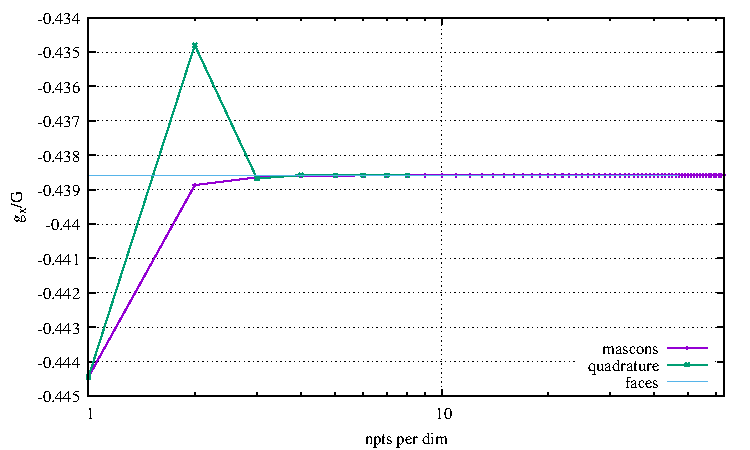
\includegraphics[width=8cm]{python_codes/fieldstone_113/results/hex_test1/gx.pdf}
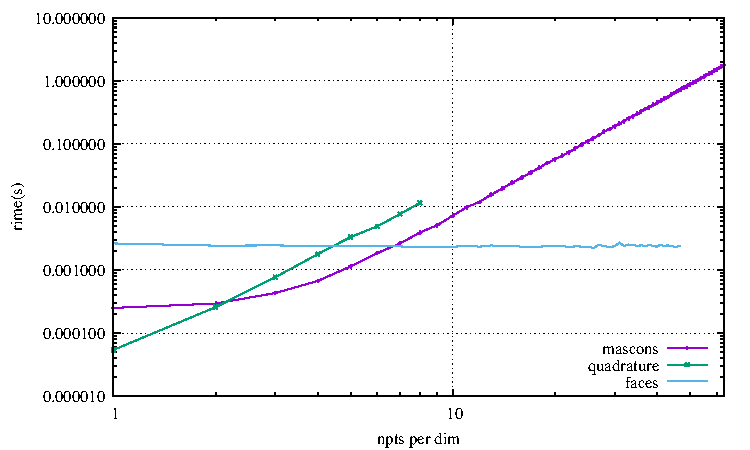
\includegraphics[width=8cm]{python_codes/fieldstone_113/results/hex_test1/time.pdf}\\
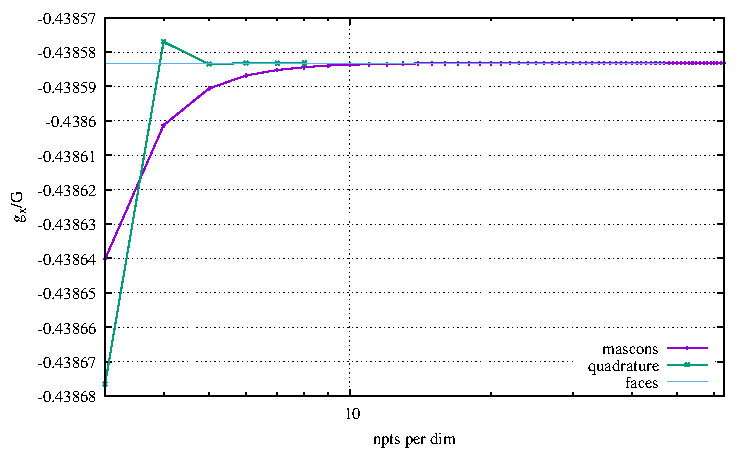
\includegraphics[width=8cm]{python_codes/fieldstone_113/results/hex_test1/gx2.pdf}
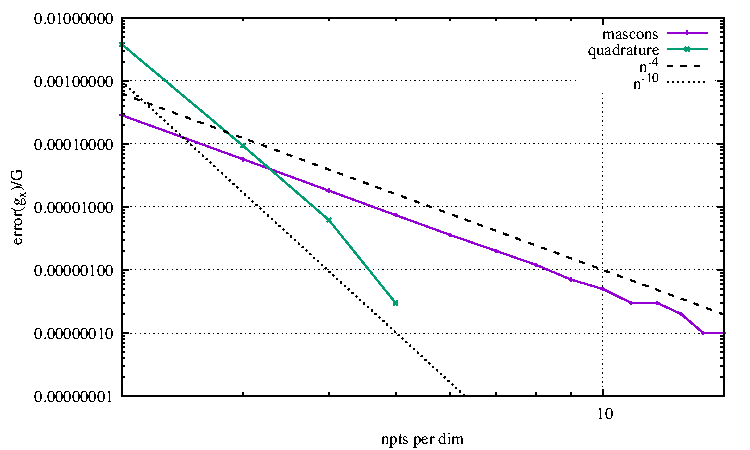
\includegraphics[width=8cm]{python_codes/fieldstone_113/results/hex_test1/gx3.pdf}\\
{\captionfont Results and cpu time for all three methods as a function of 
the used number of points (per dimension).}
\end{center}

Obviously one does not need to run the 
{\python compute\_gravity\_hexahedron\_mascons} function for every value of {\python n\_per\_dim}
since it does not depend on it, but it allows for easier plotting and a sense of the 
expected variation in the timing measurement from call to call. 

Although none of the functions have been written with efficiency in mind, 
we can look at the cpu time needed and we find that the {\python faces}
approach is fastest for {\python n\_per\_dim}$\ge 8$.
Looking at the accuracy we see that the mascons is the least accurate at low 
{\python n\_per\_dim}. Gauss quadrature becomes reasonably accurate for 
{\python n\_per\_dim}=6. 
Looking at the error convergence (where the value obtained with the faces approach is used 
as reference) we see that the quadrature approach converges much faster than the mascons approach.


%===============================================================
\section*{Hexahedron test 2: the dyke}

This originates in \textcite{uwms19} (2019). 
It consists of a dyke with a density difference 
of $+170 \si{\kg\per\cubic\meter}$, and a model space of 
$2\si{\km} \times  2 \si{\km} \times 2 \si{\km}$  was employed. 
The dyke model extends from 0.2 to 0.9 km depth (the coordinates
of all 8 vertices is given in the article). The 3-D view of buried dyke is shown here:

\begin{center}
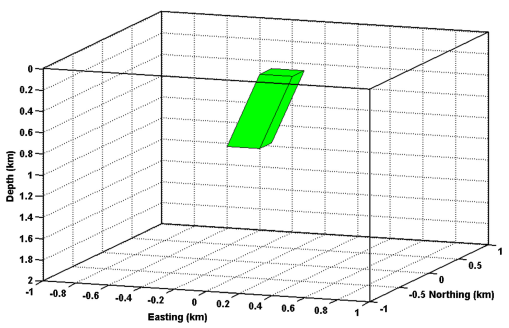
\includegraphics[height=3.5cm]{python_codes/fieldstone_113/images/uwms19_a}
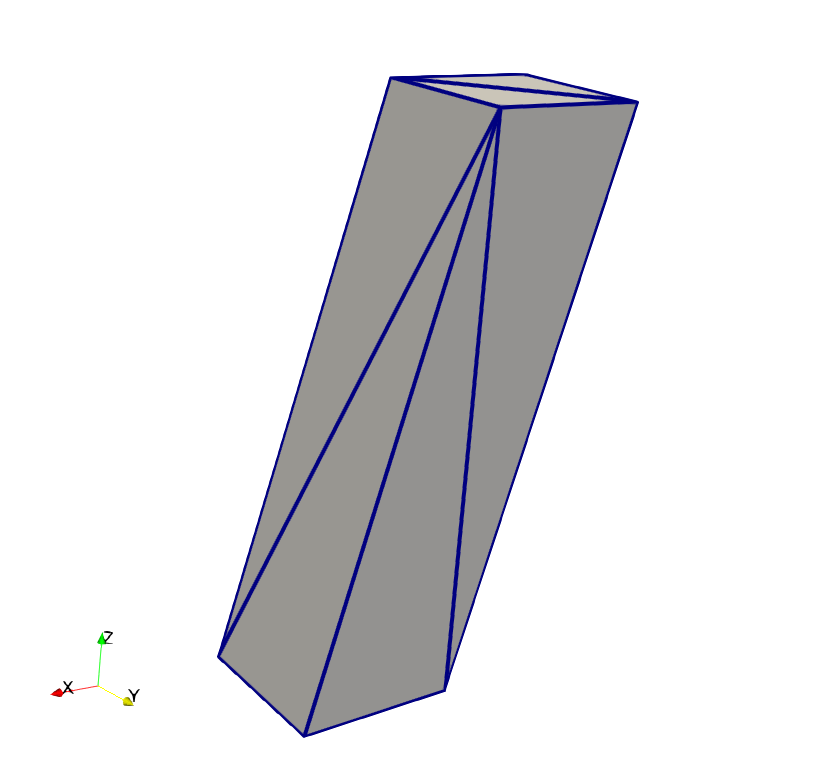
\includegraphics[height=3.5cm]{python_codes/fieldstone_113/images/dyke}\\
{\captionfont Left: figure from the paper; Right: Paraview rendering.}
\end{center}

In the paper a $11 \times 11$ grid in the horizontal plane with observation
points at 0.1-km intervals was used. The gravity anomaly
was calculated using the Gauss-Legendre integration, and calculation result is shown below:

\begin{center}
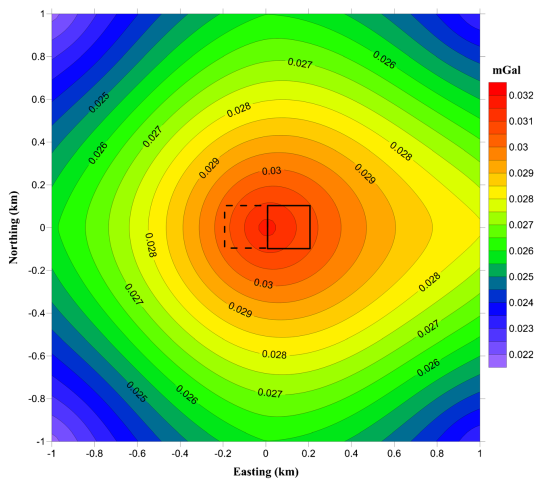
\includegraphics[width=5cm]{python_codes/fieldstone_113/images/uwms19_b}\\
{\captionfont Surface gravity anomaly distribution for the inclined dyke
block with the density difference of $+170 \si{\kg\per\cubic\meter}$.}
\end{center}

At this stage, looking at the figure above, I have my doubts: given the orientation of
the hexahedron (look at the dashed line) why is gravity higher on the other side of it?
(check the yellow 'ring'). Something is off, and this is corroborated by my own 
measurements which yield the same field for all three methods (so only one is shown): 

\begin{center}
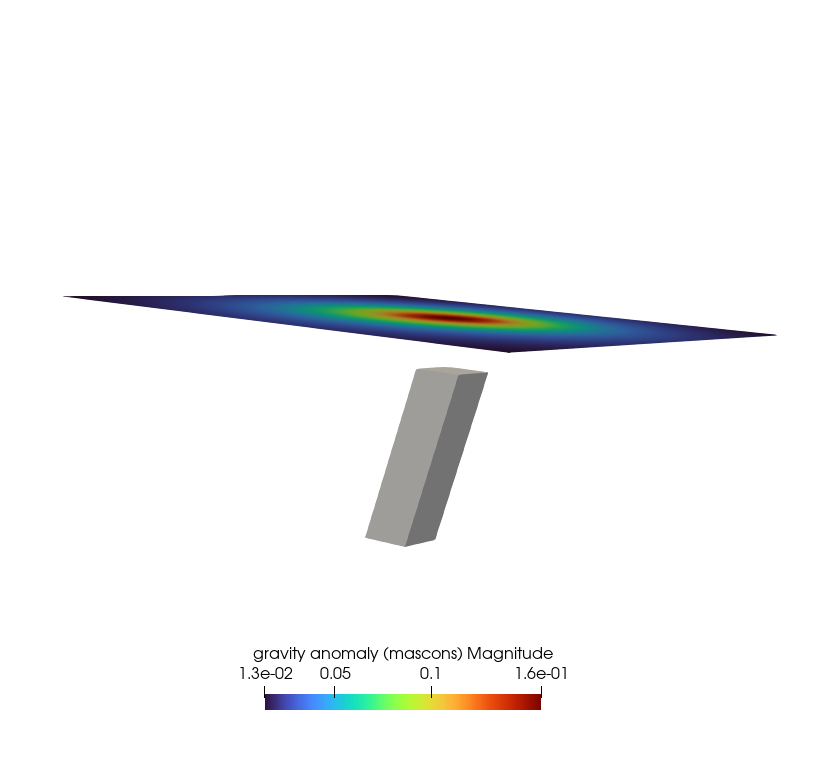
\includegraphics[width=5.7cm]{python_codes/fieldstone_113/results/hex_test2/ggg1}
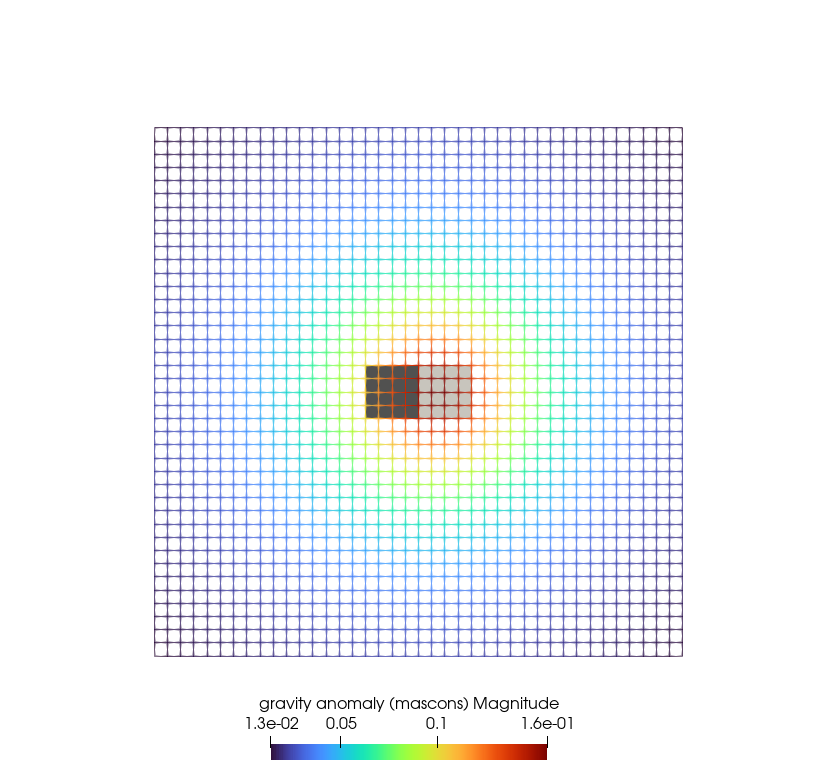
\includegraphics[width=5.7cm]{python_codes/fieldstone_113/results/hex_test2/ggg2}
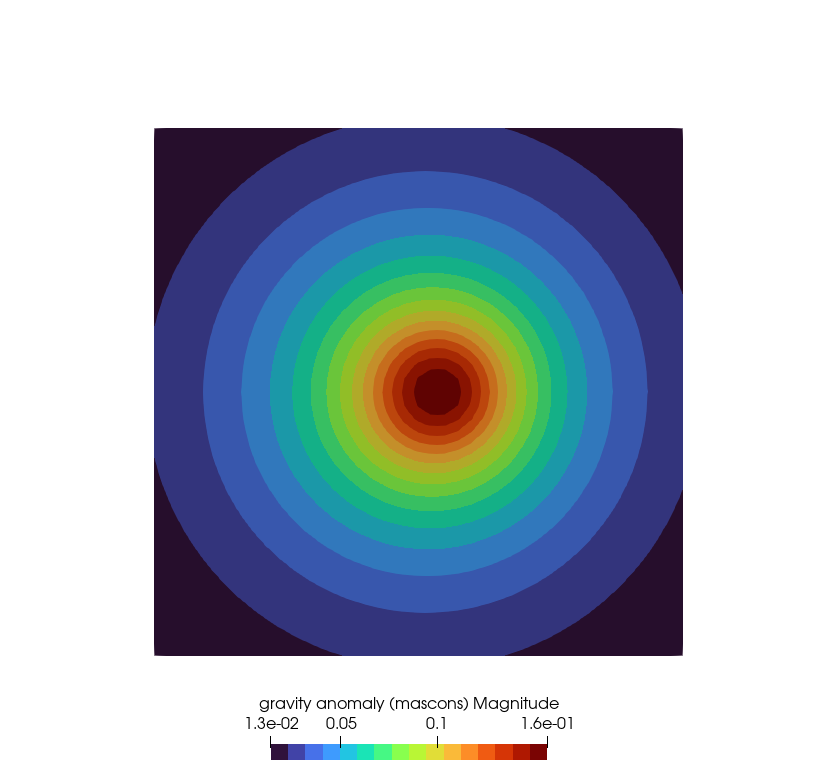
\includegraphics[width=5.7cm]{python_codes/fieldstone_113/results/hex_test2/ggg3}\\
{\captionfont Results obtained in mGal. The asymmetry in the surface signal is not very pronounced.}
\end{center}

%===============================================================
\section*{Hexahedron test 3: two buried blocks}

This also originates in \textcite{uwms19} (2019). The coordinates of
the vertices for both blocks are given in Table 2 of the publication.

\begin{center}
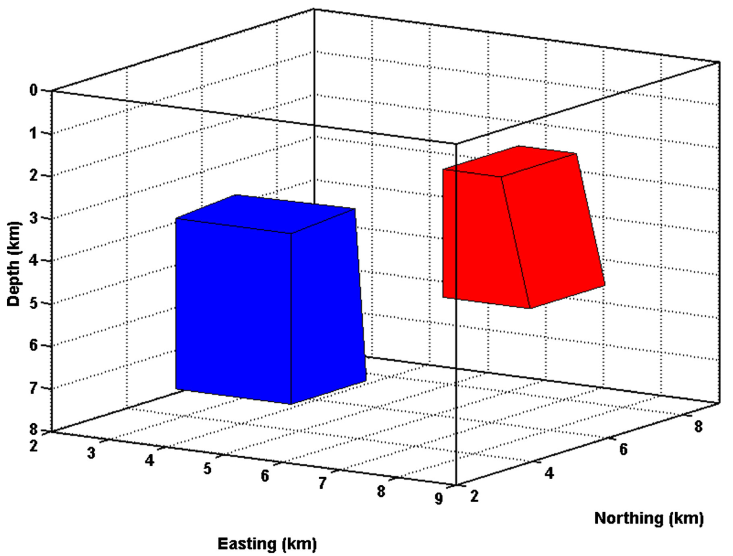
\includegraphics[width=7cm]{python_codes/fieldstone_113/images/uwms19_c}
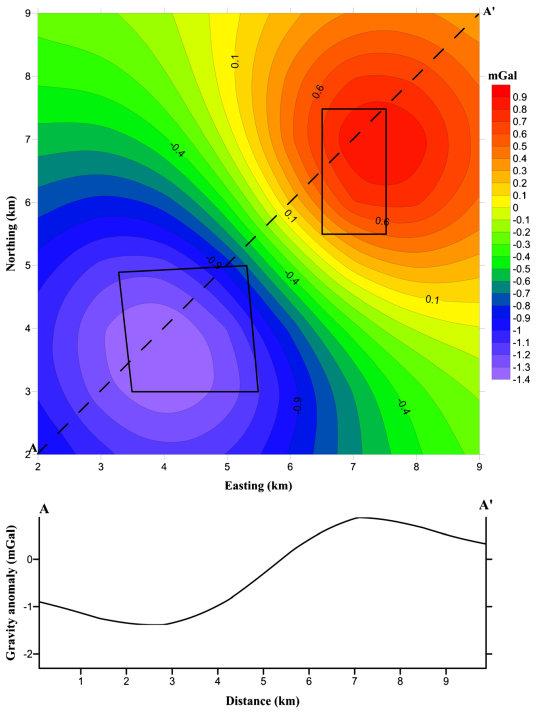
\includegraphics[width=5cm]{python_codes/fieldstone_113/images/uwms19_d}\\
{\captionfont Left: Two blocks model with different densities. The red block 
has positive density difference ($+400~\si{\kg\per\cubic\meter}$), and blue block has negative density
difference ($-400~\si{\kg\per\cubic\meter}$). Right: Surface gravity anomaly map (top) for the 
buried blocks with different densities and the gravity profile (bottom) along the A-A' line.
Since the values range from negative to positive, this is likely the $g_z$
component that is shown, not $|\vec{g}|$.}
\end{center}

\begin{center}
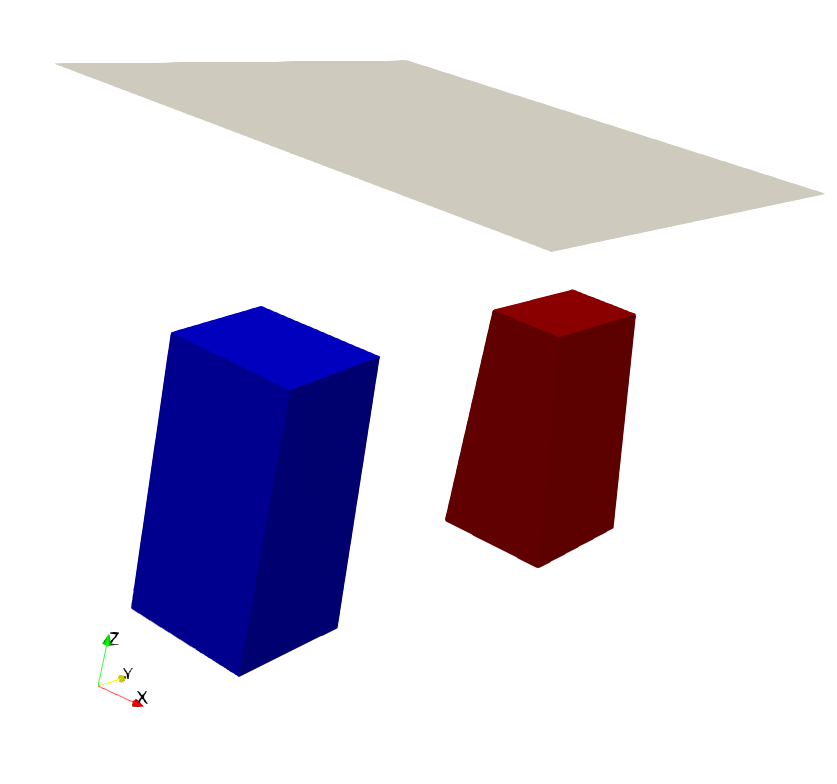
\includegraphics[width=6cm]{python_codes/fieldstone_113/images/blocks_1}
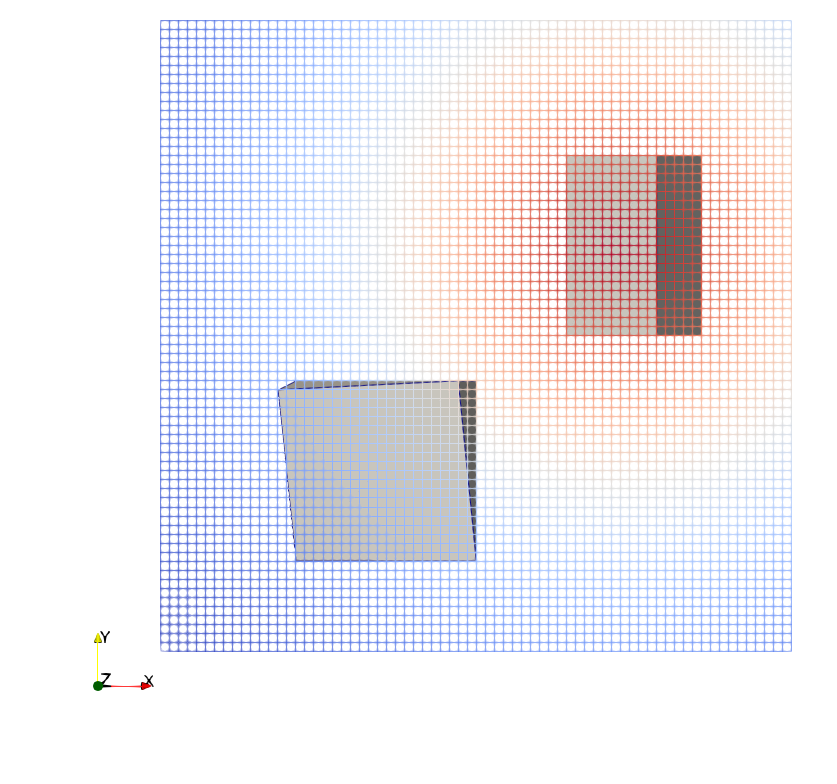
\includegraphics[width=6cm]{python_codes/fieldstone_113/images/blocks_2}
\end{center}

I use $10^3$ mascons and $7^3$ quadrature points in what follows.
We find that all methods yield very similar results and that the range
of values matches the one in the publication: 

\begin{center}
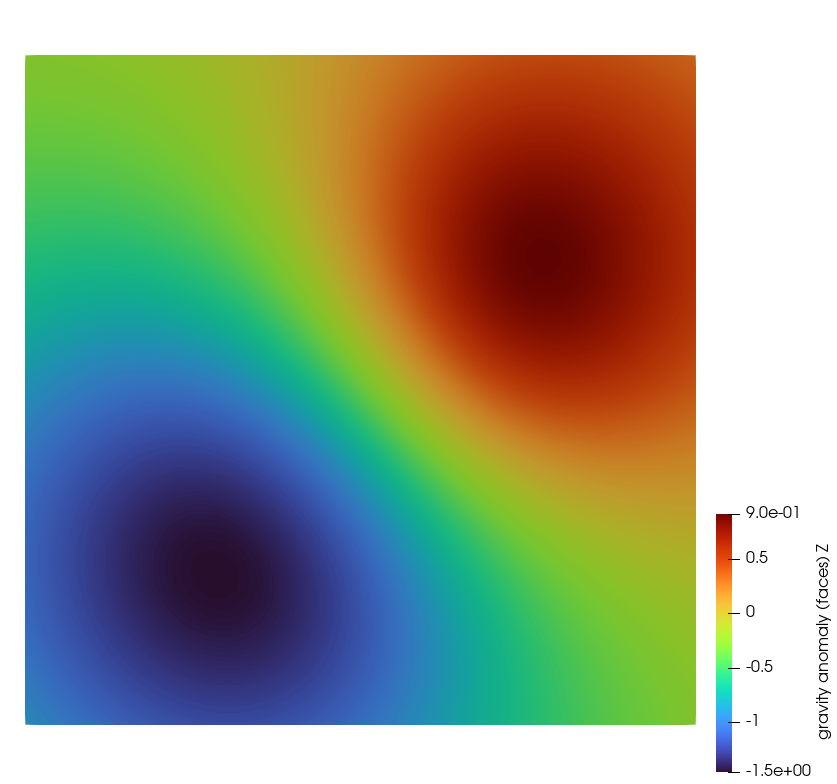
\includegraphics[width=5.7cm]{python_codes/fieldstone_113/results/hex_test3/g_faces}
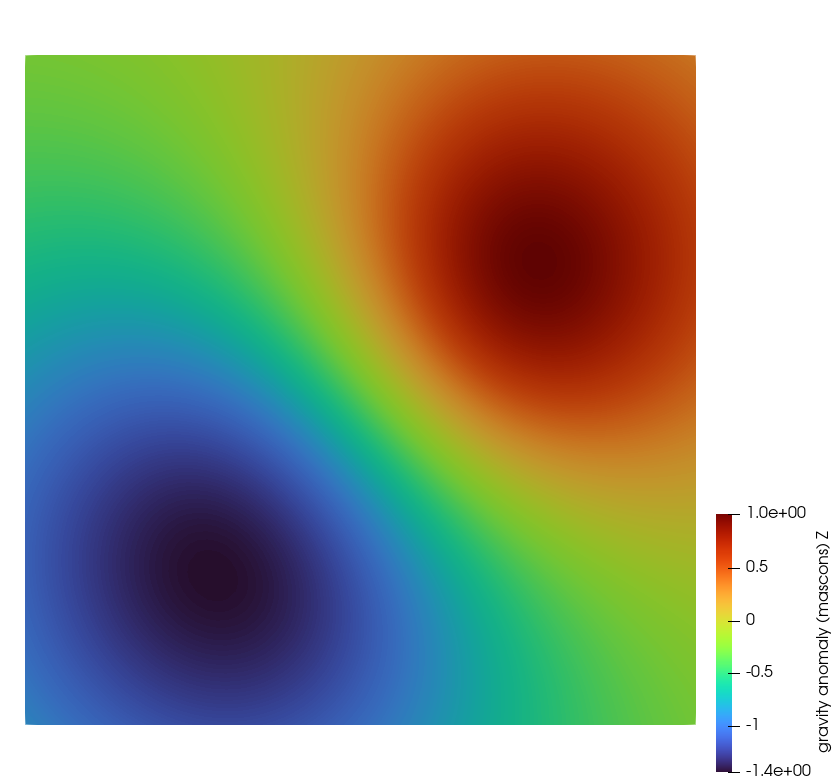
\includegraphics[width=5.7cm]{python_codes/fieldstone_113/results/hex_test3/g_mascons}
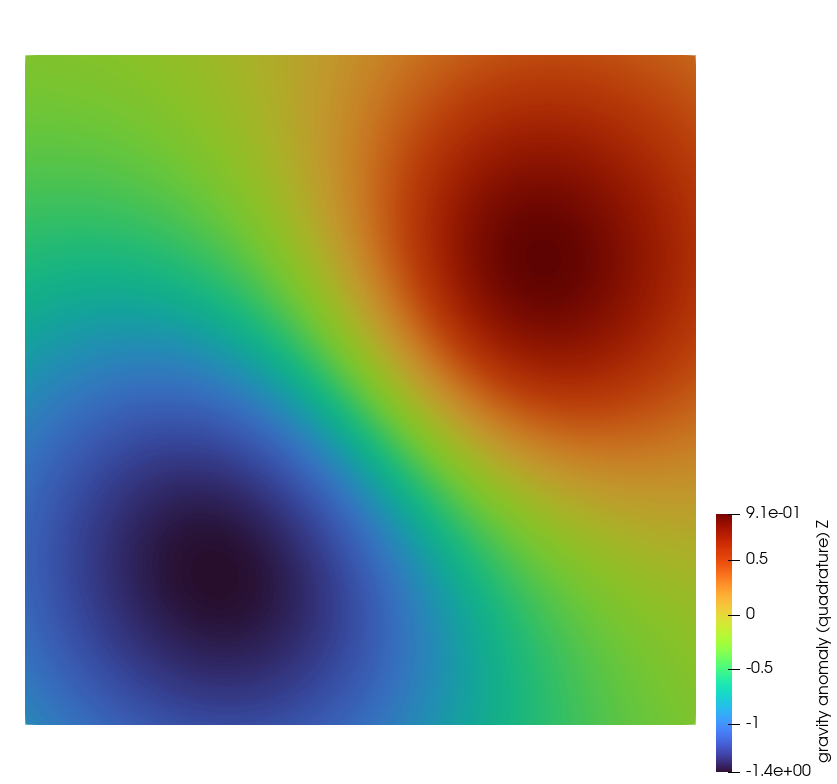
\includegraphics[width=5.7cm]{python_codes/fieldstone_113/results/hex_test3/g_quadrature}\\
{\captionfont $g_z$ Results obtained on a $71\times71$ grid. From left to right: 
faces, mascons, quadrature.}
\end{center}

Looking at the $A-A'$ section we see that the 'naive' mascons results are 
a bit off with regards to the other two methods and the 'fancy' mascons method.
Note that the mascons2 function is much slower than the others.

\begin{center}
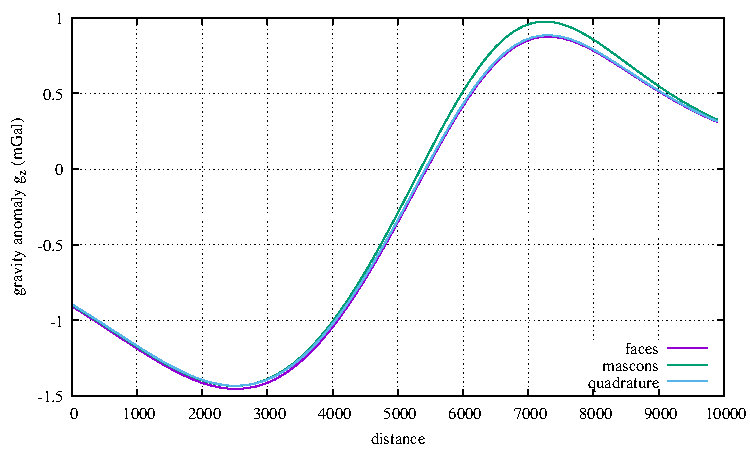
\includegraphics[width=8cm]{python_codes/fieldstone_113/results/hex_test3/line.pdf}\\
{\captionfont $g_z$ on the A-A' line of the figure above.}
\end{center}


%===============================================================
\section*{Hexahedron test 4: the irregular hexahedron}

This is a simple test which I have designed. The hexahedron is such that 
none of its faces is a plane, and that opposite faces are obviously 
not parallel. I created this test when I was investigated why the 'naive'
mascons did not yield identical results as the other 2 methods and this lead me 
to write the 'clever' mascons approach.

\begin{center}
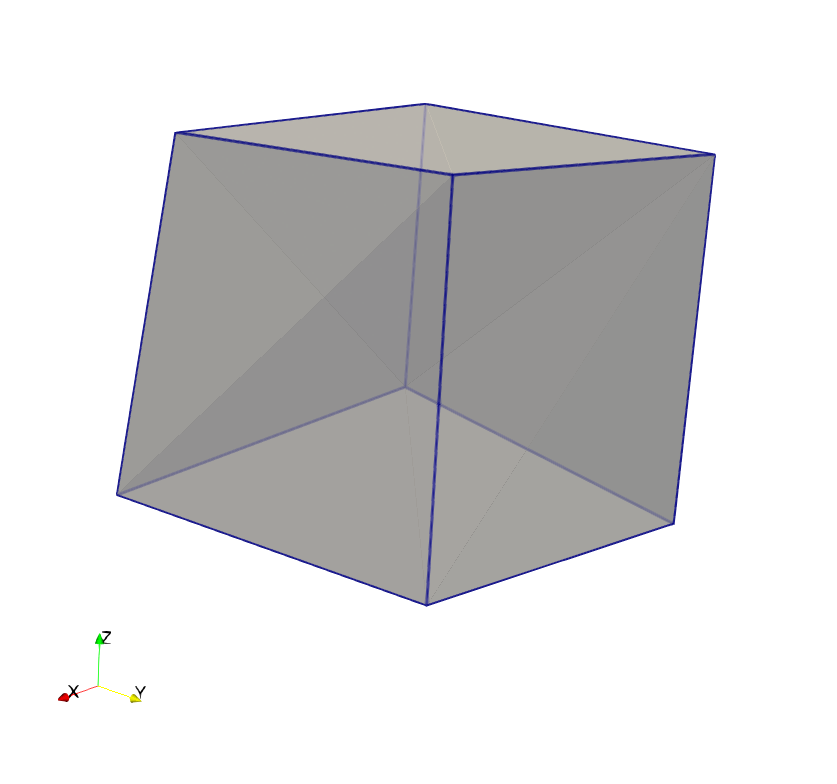
\includegraphics[width=5.7cm]{python_codes/fieldstone_113/results/hex_test4/myblock_2}
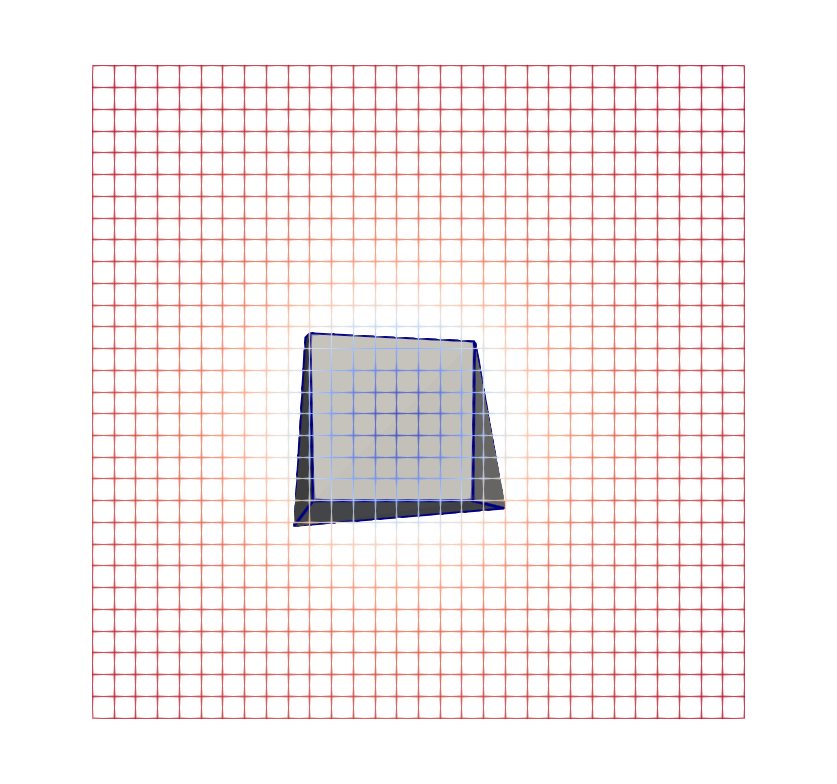
\includegraphics[width=5.7cm]{python_codes/fieldstone_113/results/hex_test4/myblock_1}
\end{center}

All three methods agree reasonably well. 

\begin{center}
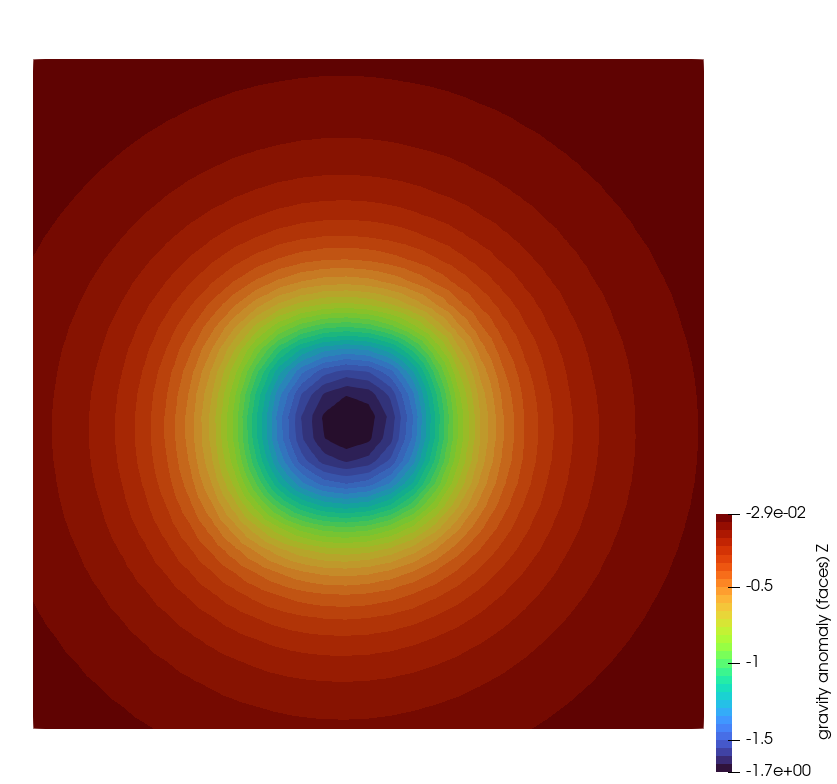
\includegraphics[width=5.7cm]{python_codes/fieldstone_113/results/hex_test4/g_faces}
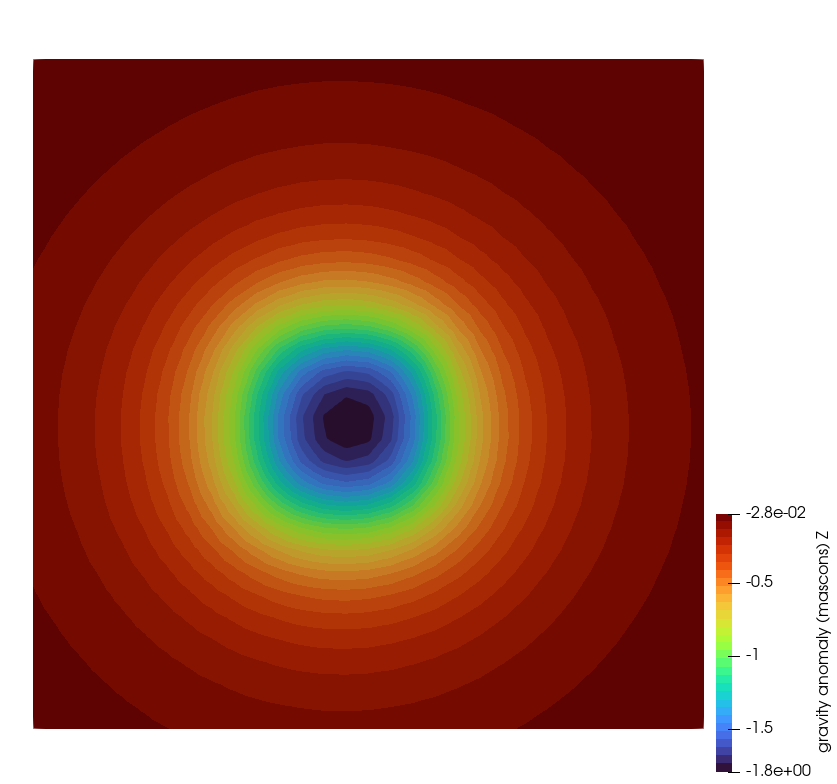
\includegraphics[width=5.7cm]{python_codes/fieldstone_113/results/hex_test4/g_mascons}
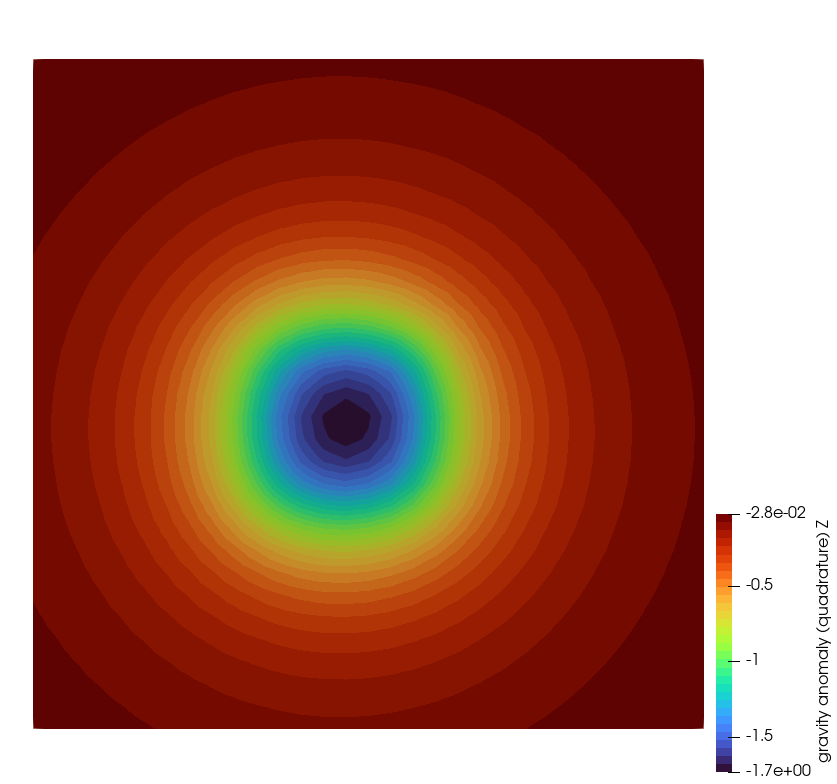
\includegraphics[width=5.7cm]{python_codes/fieldstone_113/results/hex_test4/g_quad}
\end{center}


%===============================================================
\section*{Hexahedron test 5: reverse faulted blocks}

This also originates in \textcite{uwms19} (2019). The coordinates of
the vertices for both blocks are given in Table 2 of the publication.

We are now dealing with a reverse faulted block with the
hanging wall located at a depth of 2 km and the footwall at a depth
of 3 km. The footwall block extends to the depth of 6.5 km, and a
uniform background density of $2600~\si{\kg\per\cubic\meter}$ is assumed with a
density contrast of $-500~\si{\kg\per\cubic\meter}$. The model space is 
$20 km \times  20 km \times 7 km$ 
in the $x-$, $y-$, and $z-$directions, respectively. 
The gravity anomaly distribution is calculated and presented in the $xy$-plane.

\begin{center}
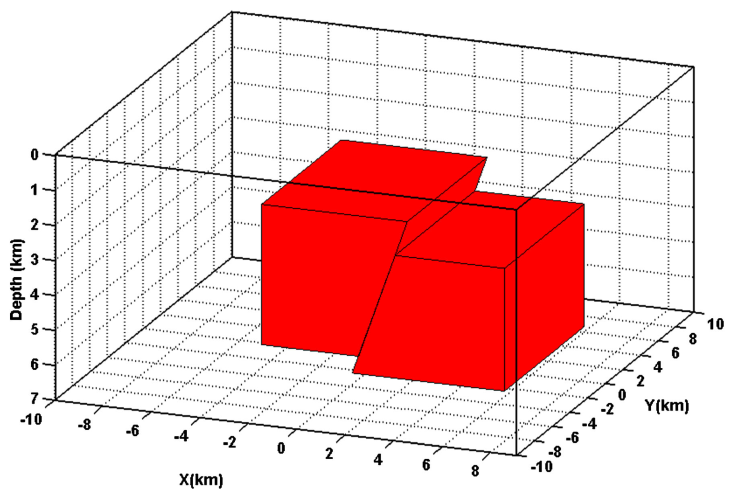
\includegraphics[width=5.7cm]{python_codes/fieldstone_113/images/uwms19_e}
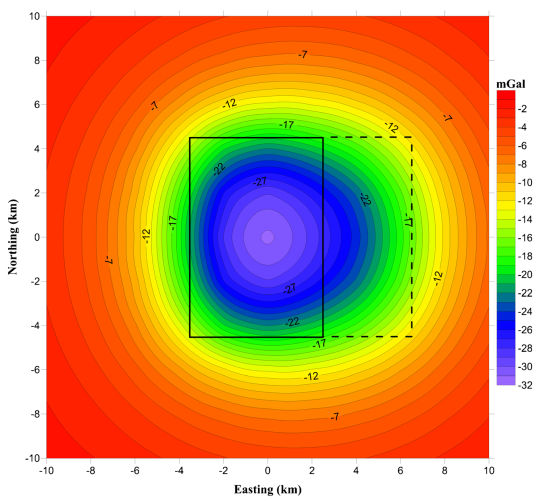
\includegraphics[width=5.7cm]{python_codes/fieldstone_113/images/uwms19_f}
\end{center}

\begin{center}
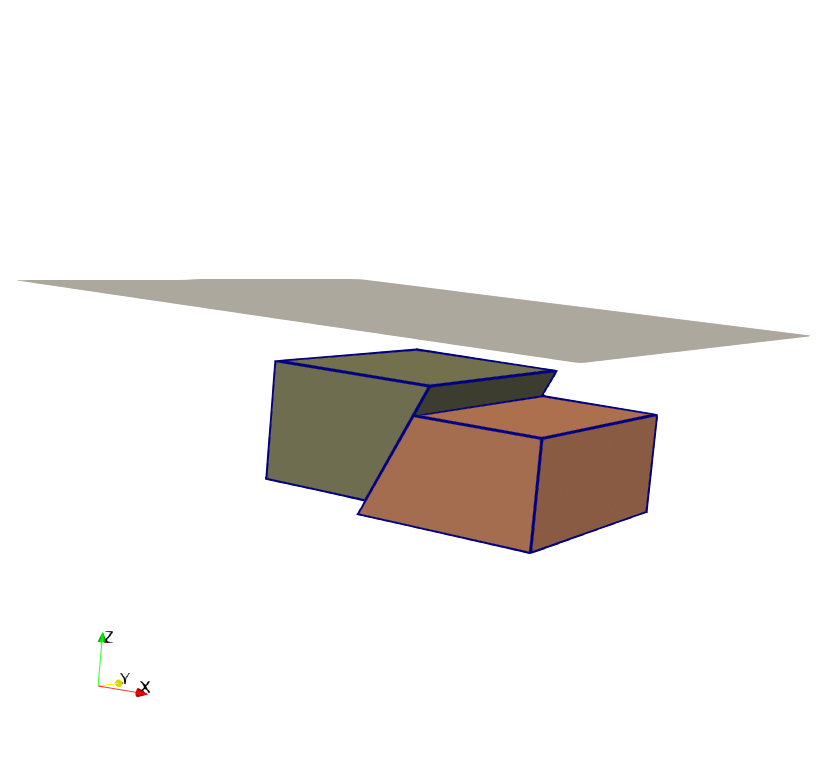
\includegraphics[width=5.7cm]{python_codes/fieldstone_113/results/hex_test5/blocks1}
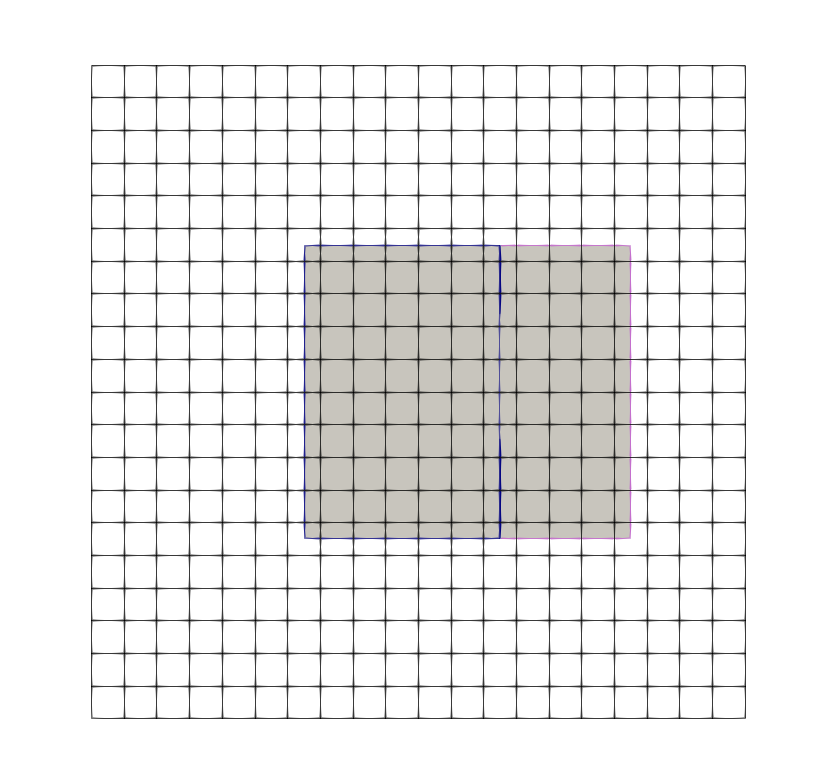
\includegraphics[width=5.7cm]{python_codes/fieldstone_113/results/hex_test5/blocks2}
\end{center}

\begin{center}
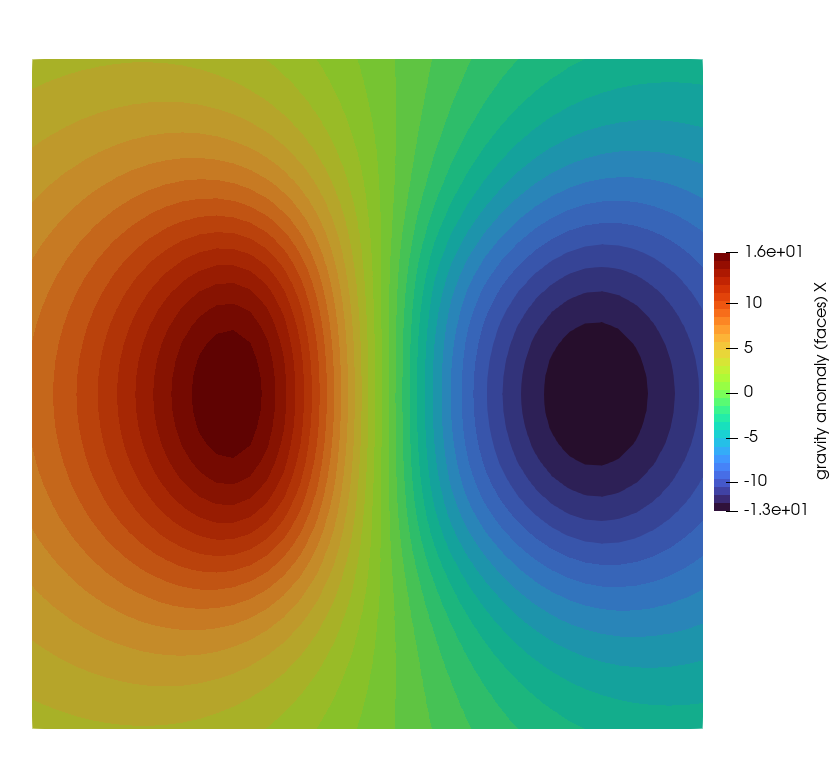
\includegraphics[width=5.7cm]{python_codes/fieldstone_113/results/hex_test5/gx}
\includegraphics[width=5.7cm]{python_codes/fieldstone_113/results/hex_test5/gy}
\includegraphics[width=5.7cm]{python_codes/fieldstone_113/results/hex_test5/gz}\\
{\captionfont Left to right: $g_x$, $g_y$ and $g_z$ components.}
\end{center}



-----------------------------

TODO:

- potential is returned by all functions but never plotted above

- compute gradients for all three methods.

- find better benchmarks. For regular cuboid, compare with function in stone 84

